% ============================================================================
% Accessibility
% ============================================================================
\DocumentMetadata{
  lang = en-US, 
  pdfstandard = ua-2, 
  tagging = on, 
  tagging-setup = {math/setup=mathml-SE}
}

% ============================================================================
% Document Properties - used on title slide and PDF metadata fields
% ============================================================================
\def\PresTitle{Precision Hand Tools}  % Required - top line of title slide
\def\PresSubtitle{Baker College Engineering}         % Optional - second line
\def\PresAuthor{Brad Peirson}               % Required - below dividing line
\def\PresInstitute{College of Information Technology and Engineering}       % Optional
\def\PresDate{}                             % Optional
\def\PresKeywords{}                         % Optional - used for hyperref

% Presentation Formatting
% ============================================================================
% ============================================================================
% Class Declaration
% ============================================================================
\documentclass[
        mode = handout,     % Projector = one bullet at a time, Handout = all
        font-size=14pt,     % Only accepts 9, 10, 12, 14, 17, 20
        pdfusetitle         % Pulls \title property from document
    ]
    {ltx-talk}              % ltx-talk class

% ============================================================================
% Custom Colors
% ============================================================================
\usepackage[table]{xcolor}
% Colors from the Baker College Style Guide
%\definecolor{BakerADARed}{RGB}{231, 0, 46}   % #e7002e Official ADA red-doesn't pass WCAG AAA for small text
\definecolor{BakerADARed}{RGB}{181, 0, 36}    % #b50024 Adjusted ADA red-passes WCAG AAA for small text
\definecolor{HoneyYellow}{RGB}{255, 196, 0}   % #ffc400
\definecolor{UpNorthGreen}{RGB}{114, 191, 68} % #72bf44
\definecolor{LakeBlue}{RGB}{134, 183, 227}    % #86b7e3
\definecolor{BakerADI}{RGB}{58, 98, 170}
\definecolor{BakerCIM}{RGB}{217, 35, 47}
\definecolor{BakerBlack}{RGB}{31, 34, 40}     % #1f2228
\definecolor{BakerWhite}{RGB}{255, 255, 255}
\definecolor{BakerRed}{RGB}{239, 0, 48}
\definecolor{Abbey}{RGB}{80, 82, 88}
\definecolor{RollingStone}{RGB}{121, 124, 126}
\definecolor{HitGray}{RGB}{165, 169, 172}
\definecolor{Iron1}{RGB}{201, 206, 209}
\definecolor{Iron}{RGB}{222, 225, 226}
\definecolor{BlackHaze1}{RGB}{237, 240, 240}
\definecolor{BlackHaze}{RGB}{245, 247, 247}

% ============================================================================
% Document Data
% ============================================================================
\title{\PresTitle}
\author{\PresAuthor}
\institute{\PresInstitute}
\date{\PresDate}

%Set up the hyperlink colors
\hypersetup{colorlinks,
    linkcolor=BakerBlack,
    urlcolor=BakerADARed,
    pdfauthor = {\PresAuthor},
    %pdftitle = {\PresentationTopic},   % Title is pulled directly
    pdfsubject = {\PresSubtitle},
    pdfkeywords = {\Keywords},
    pdfcreator = {LaTeX with hyperref package},
    pdfproducer = {LuaLaTeX}
    }

% Map your custom style guide colors to the progress bar aliases
\colorlet{pbcomplete}{BakerADARed}
\colorlet{pbincomplete}{Iron}

\usepackage[most]{tcolorbox}

% ============================================================================
% Footer Format
% ============================================================================
\EditInstance{footer}{std}{
  color         = Abbey,
  separator     = \hfill,
  element-order = {title, institute, framenumber},
  right-hspace  = 3mm,
  left-hspace   = 3mm,
}

% \DeclareInstance{footer}{empty}{
%   element-order = {}
% }

% ============================================================================
% Progress Bar Toggles & Helper Macros
% ============================================================================
\usepackage{xfp}        % Needed for floating point math
\newif\ifprogressbar    % Used to determine whether or not to show the bar
\progressbartrue        % Set the bar to true at the start

% Helper macro to automatically turn off the progress bar inside title/section frames
\newcommand{\makeblindframe}[1]{%
  \progressbarfalse
  #1%
  \progressbartrue
}

% ============================================================================
% Custom Page Formats
% ============================================================================
\let\oldmaketitle\maketitle         % Backup the original maketitle command
\let\oldsection\section             % Backup the original section command
\let\oldsubsection\subsection       % Backup the original subsection command

\makeatletter
\renewcommand{\maketitle}{%
\makeblindframe{%
  \disableglobalbackground
  \slidebackground{PresentationTitleGraphic_2048x1151}%
  \color{white}%
  %\UseInstance{footer}{wallpaper}
  \begin{frame}[wallpaper]
    \vspace*{1in}%
      \begin{tcolorbox}[
          enhanced,
          colback=black,       
          colframe=black,      
          opacityfill=0.25,       
          arc=6pt,                
          boxrule=0pt,            
          left=20pt, right=20pt,  
          top=20pt, bottom=20pt,
          width=0.80\textwidth,   
          halign=left             
      ]
          \color{white}%
          % Title (Always visible)
          {\large\bfseries\sffamily \@title}\\[0.5em]%
          
          % Conditional Subtitle
          \ifx\PresSubtitle\empty
          \else
            {\normalsize\sffamily \PresSubtitle}\\[0.5em]%
          \fi
          
          % High-contrast divider line
          {\color{white!80}\rule{0.3\textwidth}{0.8pt}}\\[0.5em]%
          
          % Author (Always visible)
          {\small\sffamily \@author}\\%
          
          % Conditional Institute
          \ifx\PresInstitute\empty
          \else
            {\small\sffamily \PresInstitute}\\%
          \fi
          
          % Conditional Date
          \ifx\PresDate\empty
          \else
            {\small\sffamily \@date}\\%
          \fi
      \end{tcolorbox}%
      \vfill     
  \end{frame}%
  \enableglobalbackground{BG}%
  \color{black}%
  %\UseInstance{footer}{std}
}%
}
\makeatother

% Create a variable container to hold the current section title
\newcommand{\currentsectiontitle}{}

% Redefine \section to take 1 argument (the title)
\renewcommand{\section}[1]{%
\makeblindframe{%
  \renewcommand{\currentsectiontitle}{#1}%
  \disableglobalbackground
  \slidebackground{PresentationSectionBackground_2048x1151}%
  \begin{frame}
    \vfill
    %\vspace*{0.625in}%
    \begin{tcolorbox}[
        enhanced,
        colback=black,       
        colframe=black,      
        opacityfill=0.25,       
        arc=6pt,                
        boxrule=0pt,            
        left=20pt, right=20pt,  
        top=20pt, bottom=20pt,
        width=0.80\textwidth,   
        halign=left             
    ]
        \color{white}%
        {\large\bfseries\sffamily #1}\\[0.5em]%   
    \end{tcolorbox}%
    \vfill 
  \end{frame}%
  \oldsection{#1}%
  \enableglobalbackground{BG}%

  % This will be used for an auto TOC at every section
  % Right now ltx-talk TOC is still in development
  % Once it comes a little further along this can be used
  % \begin{frame}
  %       \frametitle{Section Overview}
  %       \tableofcontents[sections=\thesection]
  %   \end{frame}%
}%
}

% Redefine \subsection to take 1 argument
\renewcommand{\subsection}[1]{%
\makeblindframe{%
  \disableglobalbackground
  \slidebackground{PresentationSectionBackground_2048x1151}%
  \begin{frame}
    \vfill
    %\vspace*{0.25in}% 
    \begin{tcolorbox}[
        enhanced,
        colback=black,       
        colframe=black,      
        opacityfill=0.25,       
        arc=6pt,                
        boxrule=0pt,            
        left=20pt, right=20pt,  
        top=20pt, bottom=20pt,
        width=0.80\textwidth,   
        halign=left             
    ]
        \color{white}%
        {\large\bfseries\sffamily\currentsectiontitle}\\[0.5em]%
        {\normalsize\sffamily #1}%
    \end{tcolorbox}%
    \vfill 
  \end{frame}%
  \oldsubsection{#1}%
  \enableglobalbackground{BG}%
}%
}

%Set the fonts to use NeueHaas Grotesk
\setsansfont{NHAASGROTESKTXPRO-}[
    Path=../NeueHaasGroteskFiles/,
    Scale=1.0,
    Extension = .ttf,
    UprightFont=*55Rg,
    BoldFont=*75Bd,
    ItalicFont=*56It,
    BoldItalicFont=*76BdIt
    ]

% Force the document default family to Sans-Serif
\renewcommand{\familydefault}{\sfdefault}

\usepackage{mathtools} % Load BEFORE unicode math settings
\setmathfont{Fira Math}[Scale=MatchLowercase] 

% 1. Turn global background ON
\newcommand{\enableglobalbackground}[1]{%
  \AddToHook{shipout/background}[mybg]{%
    \put(0, -\paperheight){%
      \includegraphics[width=\paperwidth, height=\paperheight, artifact]{#1}%
    }%
  }%
}

% 2. Turn global background OFF
\newcommand{\disableglobalbackground}{%
  \RemoveFromHook{shipout/background}[mybg]%
}

\newcommand{\slidebackground}[1]{%
  \AddToHookNext{shipout/background}{%
    \put(0, -\paperheight){%
      \includegraphics[width=\paperwidth, height=\paperheight, artifact]{#1}%
    }%
  }%
}

% --- GLOBAL BULLET OVERRIDES ---
\renewcommand{\labelitemi}{\color{BakerBlack}\Large\textbullet}
\renewcommand{\labelitemii}{\color{BakerBlack}\large\textbullet}
\renewcommand{\labelenumi}{\color{BakerBlack}\bfseries\arabic{enumi}.}
\renewcommand{\labelenumii}{\color{BakerBlack}\bfseries\alph{enumii})}

\AddToHook{begindocument/before}{%
  \EditInstance{item}{description}{
    label-format = \normalfont\bfseries\color{BakerADARed}#1
  }%
}

\AddToHook{begindocument/before}{%
  \EditInstance{item}{basic}{
    label-format = \color{BakerADARed}#1
  }%
}

% Global override for ltx-talk slide titles
\EditInstance{frametitle}{header}{
    font = \rule{0pt}{1.5cm}\bfseries\Large,
}

\EditInstance{header}{std}{
    font = \bfseries\huge,
    color = BakerBlack,
}

\AddToHook{env/block/begin}{%
  \colorlet{structure}{BakerADARed}%
}

\pretocmd{\tableofcontents}{\begin{minipage}{\textwidth} \linespread{1.4}}{}{}
\apptocmd{\tableofcontents}{\end{minipage}}{}{}

%Biber not functional in ltx-talk as of 2026-05-29
%Package that allows the creation of bibliographies
\usepackage[
    backend=biber,
    style=authoryear,
    sorting=none,
    %entryhead=false
    ]{biblatex}

%Load the bibliography file
\addbibresource{../../reference.bib}

\defbibheading{bibslide}{References}

\newcolumntype{L}[1]{>{\raggedright\let\newline\\\arraybackslash\hspace{0pt}}m{#1}}
\newcolumntype{C}[1]{>{\centering\let\newline\\\arraybackslash\hspace{0pt}}m{#1}}
\newcolumntype{R}[1]{>{\raggedleft\let\newline\\\arraybackslash\hspace{0pt}}m{#1}}

%All of the graphics are in a seperate folder, this makes it so the folder doesn't have to be repeated every time
\graphicspath{
  {../assets/images}
  {../assets/diagrams}
  {../assets/plots}
}

\makeatletter
% New counter to hold the custom "max frames" for the progress bar
\newcommand{\pb@maxtotal}{1}

% Read the custom total from the .aux file if it exists
\AtBeginDocument{%
  \ifdefined\pb@storedtotal
    \let\pb@maxtotal\pb@storedtotal
  \else
    % Fallback to standard total if our custom hook hasn't run yet
    \edef\pb@maxtotal{\@totalframes}%
  \fi
}

% Custom Appendix command that caps the progress bar and turns it off
\newcommand{\talkappendix}{%
  % 1. Write the CURRENT frame number to the .aux file as the progress total
  \immediate\write\@auxout{\string\gdef\string\pb@storedtotal{\@framenumber}}%
  % 2. Turn off the progress bar for all subsequent appendix slides
  \progressbarfalse
}
\makeatother

% ============================================================================
% Progress Bar Logic 
% ============================================================================
\makeatletter               
\AddToHook{shipout/background}{%
  \ifprogressbar
    % Read ltx-talk's internal frame counter safely
    \edef\currentframe{\@framenumber}%
    \edef\totalframes{\pb@maxtotal}% Use our custom max total instead
    
    % Fallback checks: If the document hasn't fully compiled yet, default to 1
    \ifx\currentframe\empty\def\currentframe{1}\fi
    \ifx\totalframes\empty\def\totalframes{1}\fi
    
    % Draw the progress bar if we have a valid total frame count
    \ifnum\totalframes>1\relax
      % Compute fraction width: (current - 1) / (total - 1)
      \edef\pbfraction{\fpeval{(\currentframe - 1) / (\totalframes - 1)}}%
      
      % Guard rails to prevent the bar from overshooting 100% on a first compile
      \ifdim\pbfraction pt>1pt\def\pbfraction{1}\fi 
      
      \edef\completewidth{\fpeval{\pbfraction * \paperwidth}}%
      \edef\incompletewidth{\fpeval{\paperwidth - \completewidth}}%
      
      % Render full-width progress bar at the top edge
      \put(0cm, -0.1cm){%
        \color{pbcomplete}\rule{\completewidth pt}{2pt}%
        \color{pbincomplete}\rule{\incompletewidth pt}{2pt}%
      }%
    \fi
  \fi
}
\makeatother

% 1. Globally shrink all caption components right as the caption engine fires
\AddToHook{cmd/@makecaption/before}{\footnotesize}

% 2. Declare and assign a blank plug to the kernel's caption label socket
\NewSocketPlug{caption/label}{nolabel}{}
\AssignSocketPlug{caption/label}{nolabel}

\usepackage{adjustbox}

\usepackage{amssymb}
\usepackage{amsmath}

\usepackage{animate}

\usepackage{calc} % Optional, but helpful for layout

\usepackage{multirow}

\usepackage{textcomp}

\usepackage[americanvoltages]{circuitikz}
\usepackage{pgfplots}
\usepackage{pgf-pie}

\usetikzlibrary{
    intersections, 
    fillbetween,
    patterns,
    decorations.pathreplacing,
    decorations.pathmorphing,
    decorations.text,
    decorations.markings,
    arrows.meta,
    arrows,
    shapes,
    shapes.geometric,
    shadows,
    calligraphy,
    backgrounds,
    intersections,
    calc,
    math,
    positioning,
    svg.path,
    shadows,
    shadows.blur
    }

\pgfplotsset{compat=1.18}

\pgfdeclarelayer{ft}
\pgfdeclarelayer{bg}
\pgfsetlayers{bg, main, ft}

% Usage: \hexpic[]{height}{Alt text}{Attribution}{image path}
\newcommand{\hexpic}[5][]{%
  \begin{figure}
    \centering
    \begin{tikzpicture}[
      baseline=(hex.base),      
      every shadow/.style={
        shadow opacity=70
        }
      ]
      \node (hex) [
        draw=white, 
        minimum size=#2, 
        regular polygon, 
        regular polygon sides=6, 
        rotate=90,
        blur shadow
      ] {};
      \begin{scope}
        \clip (hex.corner 1) -- (hex.corner 2) -- (hex.corner 3) -- 
              (hex.corner 4) -- (hex.corner 5) -- (hex.corner 6) -- cycle;
        \node at (hex.center) [#1] {
          \includegraphics[height=#2, alt={#3}]{#5}
        };
      \end{scope}
    \end{tikzpicture}

    \vspace{0.5em}
    {\tiny #4\par}
  \end{figure}  
}

% Usage: \shadowpic[]{width}{Alt text}{Attribution}{image path}
\newcommand{\shadowpic}[5][]{%
  \begin{figure}
    \centering
    \begin{tikzpicture}
      [every shadow/.style={
        shadow opacity=70
        }
      ]
      \node (image) [
        inner sep=0,
        blur shadow
      ] {\includegraphics[width=#2, alt={#3}]{#5}};
    \end{tikzpicture}

    \vspace{0.5em}
    {\tiny #4\par}
  \end{figure}
}

\tikzset{middlearrow/.style={
        decoration={markings, 
        mark= at position 0.5 with {\arrow{#1}},
        },
        postaction={decorate}
    }
}

% Usage: \tikztodo[width]{height}{description/notes}
\newcommand{\tikztodo}[3][0.8\textwidth]{%
  \begin{center}
    \fbox{%
      \parbox[c][#2][c]{#1}{%
        \centering
        \textbf{\textcolor{red}{TODO: TikZ Diagram}}\\[0.5em]
        \small #3%
      }%
    }%
  \end{center}%
}

% Macro: \drawrails{<number_of_1cm_segments>}
\newcommand{\drawrails}[1]{
  % Calculate total depth: 1 cm per segment
  \pgfmathsetmacro{\railheight}{-1 * #1}
  
  % L1 Rail (x = 0)
  \draw[thick] (0, 0) -- (0, \railheight cm);
    
  % L2 Rail (x = 15)
  \draw[thick] (15, 0) -- (15, \railheight cm);
}

\newcommand{\ccwplus}{%
  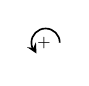
\begin{tikzpicture}[baseline=(char.base)]
    \node(char) at (0,0) {\(\scriptscriptstyle +\)};
    \draw[->, >=stealth, semithick] (0.2,0) arc (0:230:0.18cm);
  \end{tikzpicture}%
}

%====================================================================================
% Timer Ladder Symbol - Could be used for TON, TOF, RTO....
%====================================================================================
\tikzset{
    TON/.pic={

        \draw[
          BakerBlack
        ]
        (0,0)
        -- ++(0,0.375)
        -- ++(3.5,0)
        coordinate[pos=0.5](-TOP)
        -- ++(0,-1.75)
        coordinate[pos=3/14](-OUT)
        coordinate[pos=0.5](-EN1)
        coordinate[pos=0.875](-DN1)
        -- ++(-3.5,0)        
        -- (0,0)
        coordinate(-IN);

        \node[
          text=BakerBlack,
          font=\bfseries,
          anchor=east
        ](pre)
        at ($(-TOP)-(0,1.75em)$)
        {{\small PRE:}};

        \node[
          text=BakerBlack,
          font=\bfseries,
          anchor=east
        ](acc)
        at ($(pre.east)-(0,1em)$)
        {{\small ACC:}};

        \coordinate (-PRE) at (pre.east); % For the preset value
        \coordinate (-ACC) at (acc.east);

        \draw[
            BakerBlack
        ]
        (-EN1)
        -- ++(0.5,0)
        coordinate(-EN2)
        node[
            text=BakerBlack,
            anchor=west
        ]
        {{\small EN}};

        \draw[
            BakerBlack
        ]
        (-DN1)
        -- ++(0.5,0)
        coordinate(-DN2)
        node[
            text=BakerBlack,
            anchor=west
        ]
        {{\small DN}};

    }
}

%====================================================================================
% Oval ladder symbol, good for ONS, RES, etc.
%====================================================================================
\tikzset{
    ONS/.pic={

        \draw[
          BakerBlack
        ]
        (0,0)
        coordinate(-IN)
        -- ++(0.75,0)
        node[
          draw=BakerBlack, 
          text=BakerBlack, 
          font=\small, 
          minimum width=1.5cm, 
          minimum height=0.75cm, 
          anchor=west, 
          rounded corners=0.25cm
          ](ons){};
        
        \draw[BakerBlack] (ons.east) -- ++(0.75,0) coordinate(-OUT);

        \coordinate(-INS) at (ons.center);
        \coordinate(-VAR) at (ons.north); 
    }
}

%====================================================================================
% Source A, Source B, Dest box
%====================================================================================
\tikzset{
    SrcDest/.pic={
      
        \draw[
          BakerBlack
        ]
        (0,0)
        coordinate(-IN)
        -- ++(0,0.375)
        -- ++(5,0)
        coordinate[pos=0.5](-TOP)
        -- ++(0,-3.25)
        coordinate[pos=3/26](-OUT)
        -- ++(-5,0)
        -- (0,0)
        coordinate(l1);

        \node[
          text=BakerBlack,
          font=\bfseries,
          anchor=west
        ](srcA)
        at (l1)
        {{\small Src A:}};

        \node[
          text=BakerBlack,
          font=\bfseries,
          anchor=west
        ](srcB)
        at ($(l1)-(0,2em)$)
        {{\small Src B:}};

        \node[
          text=BakerBlack,
          font=\bfseries,
          anchor=west
        ](dest)
        at ($(srcB.west)-(0,2em)$)
        {{\small Dest:}};

        \coordinate(-SRCA) at (srcA.east);
        \coordinate(-AVAL) at ($(srcA.east)-(0,1em)$);
        \coordinate(-SRCB) at (srcB.east);
        \coordinate(-BVAL) at ($(srcB.east)-(0,1em)$);
        \coordinate(-DEST) at ($(-BVAL)-(0,1em)$);
        \coordinate(-DVAL) at ($(-DEST)-(0,1em)$);
    }
}

%====================================================================================
% Source A, Source B box
%====================================================================================
\tikzset{
    SrcAB/.pic={
      
        \draw[
          BakerBlack
        ]
        (0,0)
        coordinate(-IN)
        -- ++(0,0.375)
        -- ++(4,0)
        coordinate[pos=0.5](-TOP)
        -- ++(0,-2.25)
        coordinate[pos=1/6](-OUT)
        -- ++(-4,0)
        -- (0,0)
        coordinate(l1);

        \node[
          text=BakerBlack,
          font=\bfseries,
          anchor=west
        ](srcA)
        at (l1)
        {{\small Src A:}};

        \node[
          text=BakerBlack,
          font=\bfseries,
          anchor=west
        ](srcB)
        at ($(l1)-(0,2em)$)
        {{\small Src B:}};

        \coordinate(-SRCA) at (srcA.east);
        \coordinate(-AVAL) at ($(srcA.east)-(0,1em)$);
        \coordinate(-SRCB) at (srcB.east);
        \coordinate(-BVAL) at ($(srcB.east)-(0,1em)$);
    }
}

%====================================================================================
% LIMIT instruction
%====================================================================================
\tikzset{
    Limit/.pic={
      
        \draw[
          BakerBlack
        ]
        (0,0)
        coordinate(-IN)
        -- ++(0,0.375)
        -- ++(4,0)
        coordinate[pos=0.5](-TOP)
        -- ++(0,-3.25)
        coordinate[pos=3/26](-OUT)
        -- ++(-4,0)
        -- (0,0)
        coordinate(l1);

        \node[
          text=BakerBlack,
          font=\bfseries,
          anchor=west
        ](srcA)
        at (l1)
        {{\small Low:}};

        \node[
          text=BakerBlack,
          font=\bfseries,
          anchor=west
        ](srcB)
        at ($(l1)-(0,2em)$)
        {{\small Test:}};

        \node[
          text=BakerBlack,
          font=\bfseries,
          anchor=west
        ](dest)
        at ($(srcB.west)-(0,2em)$)
        {{\small High:}};

        \coordinate(-LO) at (srcA.east);
        \coordinate(-LOV) at ($(srcA.east)-(0,1em)$);
        \coordinate(-TEST) at (srcB.east);
        \coordinate(-TESTV) at ($(srcB.east)-(0,1em)$);
        \coordinate(-HI) at ($(-TESTV)-(0,1em)$);
        \coordinate(-HIV) at ($(-HI)-(0,1em)$);
    }
}

%====================================================================================
% Source Destination box
%====================================================================================
\tikzset{
    SrcSingle/.pic={
      
        \draw[
          BakerBlack
        ]
        (0,0)
        coordinate(-IN)
        -- ++(0,0.375)
        -- ++(6,0)
        coordinate[pos=0.5](-TOP)
        -- ++(0,-2.25)
        coordinate[pos=1/6](-OUT)
        -- ++(-6,0)
        -- (0,0)
        coordinate(l1);

        \node[
          text=BakerBlack,
          font=\bfseries,
          anchor=west
        ](srcA)
        at (l1)
        {{\small Source:}};

        \node[
          text=BakerBlack,
          font=\bfseries,
          anchor=east
        ](srcB)
        at ($(srcA.east)-(0,2em)$)
        {{\small Dest:}};

        \coordinate(-SRC) at (srcA.east);
        \coordinate(-SRCV) at ($(srcA.east)-(0,1em)$);
        \coordinate(-DEST) at (srcB.east);
        \coordinate(-DESTV) at ($(srcB.east)-(0,1em)$);
    }
}

%====================================================================================
% Compute Box
%====================================================================================
\tikzset{
    CPT/.pic={
      
        \draw[
          BakerBlack
        ]
        (0,0)
        coordinate(-IN)
        -- ++(0,0.375)
        -- ++(8.5,0)
        coordinate[pos=0.5](-TOP)
        -- ++(0,-1.75)
        coordinate[pos=3/14](-OUT)
        -- ++(-8.5,0)
        -- (0,0)
        coordinate(l1);

        \node[
          text=BakerBlack,
          font=\bfseries,
          anchor=west
        ](srcA)
        at (l1)
        {{\small Source:}};

        \node[
          text=BakerBlack,
          font=\bfseries,
          anchor=east
        ](srcB)
        at ($(srcA.east)-(0,2em)$)
        {{\small Exp:}};

        \coordinate(-DEST) at (srcA.east);
        \coordinate(-DESTV) at ($(srcA.east)-(0,1em)$);
        \coordinate(-EXP) at (srcB.east);
        \coordinate(-EXPV) at ($(srcB.east)-(0,1em)$);
    }
}

% ============================================================================
% Document Content
% ============================================================================
\begin{document}

\maketitle              % Redefined in the preamble to generate a full frame

\begin{frame}
    \frametitle{Agenda}
    \begingroup
        % Tighten the spacing between paragraphs/TOC lines
        \setlength{\parskip}{0.3em} 
        
        % Optionally tighten the line spacing within an entry
        %\baselineskip=1.2em 
        
        \setcounter{tocdepth}{1} % Show only sections
    \tableofcontents
    \setcounter{tocdepth}{2} % Reset back to default so subsections are tracked
    \endgroup
\end{frame}

\section{Vernier Instruments}

\begin{frame}
	\frametitle{Vernier Instruments Applications}

    \begin{columns}
        \begin{column}{0.48\linewidth}
            \begin{itemize}[<+- | alert@+>]
                \item{Vernier is a type of scale}
                \item{Used on \textbf{many} different measurement devices}
                    \begin{itemize}
                        \item{Including some micrometers}
                    \end{itemize}
            \end{itemize}
        \end{column}
        \begin{column}{0.48\linewidth}
            \hexpic[]{0.875\linewidth}{A close-up view of a metal vernier caliper positioned against a red textured background, showing lower external measuring jaws, upper internal measuring jaws, a top locking thumbscrew, and a vernier scale labeled 0.02 mm aligned with main beam millimeter graduations.}{\textbf{Attibution:} ArtMechanic, \href{https://creativecommons.org/licenses/by-sa/3.0/}{CC BY-SA 3.0}, via \href{https://commons.wikimedia.org/wiki/File:Messschieber.jpg}{Wikimedia Commons}}{Messschieber}
        \end{column}
    \end{columns}
\end{frame}

\begin{frame}
	\frametitle{Transition to Dial Tools}

    \begin{columns}
        \begin{column}{0.48\linewidth}
            Most vernier instruments were replaced by dial instruments \emph{LONG} ago...
        \end{column}
        \begin{column}{0.48\linewidth}
            \shadowpic[]{\linewidth}{A stainless steel dial caliper lying horizontally on a dark wood surface, featuring a large circular analog dial face, upper internal measurement jaws, lower external measurement jaws, a fine-adjustment thumb wheel, and a long linear beam scale.}{}{DialCaliper}
        \end{column}
    \end{columns}
\end{frame}

\begin{frame}
	\frametitle{Shift to Digital Calipers}

    \begin{columns}
        \begin{column}{0.48\linewidth}
            ...so long ago that most dial instruments have been replaced by digital instruments.
        \end{column}
        \begin{column}{0.48\linewidth}
            \shadowpic[]{\linewidth}{A digital electronic caliper lying against a plain white background with its LCD display showing a measurement reading of 11.58 mm. The tool features a stainless steel main beam marked with yellow millimeter graduations up to 150 mm, upper internal jaws, lower external jaws, control buttons for unit switching and zeroing, and a depth measuring rod extending from the right tip.}{\textbf{Attibution:} Jacek Halicki, \href{https://creativecommons.org/licenses/by-sa/4.0/}{CC BY-SA 4.0}, via \href{https://commons.wikimedia.org/wiki/File:2020_Suwmiarka_cyfrowa.jpg}{Wikimedia Commons}}{2020_Suwmiarka_cyfrowa}
        \end{column}
    \end{columns}
\end{frame}

\begin{frame}
	\frametitle{Why Use Dial Instruments?}

    When possible, you should still shoot for dial instruments\dots why?
\end{frame}

\begin{frame}
	\frametitle{Reliability of Dial Calipers}

    \shadowpic[]{0.25\linewidth}{A close-up view of the flat positive surface of a round metallic maxell CR2032 H 3 V coin cell battery. Text on the face reads maxell CR2032 H, 3 V, a large positive plus symbol in the center, and Hitachi Maxell, Ltd. Japan along the bottom curve.}{\textbf{Attibution:} \textcopyright Raymond Spekking, \href{https://creativecommons.org/licenses/by-sa/4.0/}{CC BY-SA 4.0}, via \href{https://commons.wikimedia.org/wiki/File:Coin_cell_CR2032_H_by_Hitachi_Maxell-7730.jpg}{Wikimedia Commons}}{Coin_cell_CR2032_H_by_Hitachi_Maxell-7730}

    \vspace{0.5em}
    \centering
    {\footnotesize Batteries die--dial calipers will always be ready to use when you need them.\par}
\end{frame}

\subsection{Reading a Vernier Scale}

\begin{frame}
	\frametitle{Scale Subdivisions Concept}
    
    \begin{itemize}[<+- | alert@+>]
        \item A \textbf{vernier scale} is a way to subdivide a larger scale
        \item The vernier scale works by measuring a percentage of the larger scale
        \item A distance on the vernier scale is one unit less than the same distance on the larger scale
        \item Huh?
    \end{itemize}    
\end{frame}

\begin{frame}
	\frametitle{5-Division Scale (1 of 6)}

    \begin{figure}
        \centering
        \resizebox{0.5\columnwidth}{!}{
            \begin{circuitikz}[
    american, 
    >={Latex[length=5mm, width=2mm]},
    alt={Main scale above labeled 0 through 5 aligned directly over a vernier scale below labeled 0 through 5. The zero mark of the vernier scale aligns perfectly with the zero mark of the main scale, and the 5 mark of the vernier scale aligns with the 4 mark of the main scale.}
    ]

    \draw[BakerBlack] (0,0) -- (5,0);
    
    \foreach \x in {0,...,5}
        \draw[BakerBlack] (\x,0) -- (\x,0.5) node[text=BakerBlack, anchor=south, align=center]{\x};

    \node[text=UpNorthGreen, anchor=south, align=center] at (2.5,1){Main Scale};
    \node[text=BakerADARed, anchor=north, align=center] at (2,-1){Vernier Scale};

    \begin{scope}
        \draw[BakerBlack] (0,-0.1) -- (4,-0.1);
        
        \foreach \x in {0,0.8,1.6,2.4,3.2,4}
            \draw[BakerBlack] (\x,-0.1) -- (\x,-0.5);

        \node[text=BakerBlack, anchor=north, align=center] at (0,-0.5){0};
        \node[text=BakerBlack, anchor=north, align=center] at (0.8,-0.5){1};
        \node[text=BakerBlack, anchor=north, align=center] at (1.6,-0.5){2};
        \node[text=BakerBlack, anchor=north, align=center] at (2.4,-0.5){3};
        \node[text=BakerBlack, anchor=north, align=center] at (3.2,-0.5){4};
        \node[text=BakerBlack, anchor=north, align=center] at (4,-0.5){5};                    
    \end{scope}
    
\end{circuitikz}
            }
    \end{figure}  
\end{frame}

\begin{frame}
	\frametitle{5-Division Scale (2 of 6)}

    \begin{figure}
        \centering
        \resizebox{0.5\columnwidth}{!}{
            \begin{circuitikz}[
    american, 
    >={Latex[length=5mm, width=2mm]},
    alt={Main scale above and vernier scale below showing four divisions on the main scale equal in total length to five divisions on the vernier scale. Double-headed arrows highlight four main scale units versus five vernier scale units.}
    ]

    \draw[BakerBlack] (0,0) -- (5,0);
    
    \foreach \x in {0,...,5}
        \draw[BakerBlack] (\x,0) -- (\x,0.5) node[text=BakerBlack, anchor=south, align=center]{\x};

    \draw[UpNorthGreen, ultra thick, shorten <=0.25cm] (0,1) -- (0,2);
    \draw[UpNorthGreen, ultra thick, shorten <=0.25cm] (4,1) -- (4,2);
    \draw[UpNorthGreen, ultra thick, <->] (0,1.5) -- node[midway, text=BakerBlack, anchor=south, align=center]{4 Divisions} (4,1.5);

    \draw[BakerADARed, ultra thick, shorten <=0.25cm] (0,-1) -- (0,-2);
    \draw[BakerADARed, ultra thick, shorten <=0.25cm] (4,-1) -- (4,-2);
    \draw[BakerADARed, ultra thick, <->] (0,-1.5) -- node[midway, text=BakerBlack, anchor=north, align=center]{5 Divisions} (4,-1.5);

    \begin{scope}
        \draw[BakerBlack] (0,-0.1) -- (4,-0.1);
        
        \foreach \x in {0,0.8,1.6,2.4,3.2,4}
            \draw[BakerBlack] (\x,-0.1) -- (\x,-0.5);

        \node[text=BakerBlack, anchor=north, align=center] at (0,-0.5){0};
        \node[text=BakerBlack, anchor=north, align=center] at (0.8,-0.5){1};
        \node[text=BakerBlack, anchor=north, align=center] at (1.6,-0.5){2};
        \node[text=BakerBlack, anchor=north, align=center] at (2.4,-0.5){3};
        \node[text=BakerBlack, anchor=north, align=center] at (3.2,-0.5){4};
        \node[text=BakerBlack, anchor=north, align=center] at (4,-0.5){5};                    
    \end{scope}
    
\end{circuitikz}
            }
        
        \vspace{0.5em}
        {\footnotesize If the main scale has 5 divisions, the Vernier scale \emph{also} have 5 divisions but will \emph{fit them} in the space of 4 divisions of the main scale.\par}
    \end{figure}  
\end{frame}

\begin{frame}
	\frametitle{5-Division Scale (3 of 6)}

    \begin{figure}
        \centering
        \resizebox{0.5\columnwidth}{!}{
            \begin{circuitikz}[
    american, 
    >={Latex[length=5mm, width=2mm]},
    alt={Main scale labeled 0 and 1 showing four intermediate division lines in red. Below it, a vernier scale shows its zero and one marks, with a green line pointing to the difference of one fifth unit between the scale divisions. An arc above highlights the length of four fifths.}
    ]

    \draw[BakerBlack] (0,0) -- (5,0);
    
    \foreach \x in {0,5}
        \draw[BakerBlack] (\x,0) -- (\x,0.5);

    \foreach \x in {1,2,3,4}
        \draw[BakerADARed] (\x,0) -- (\x,0.5);

    \node[text=BakerBlack, anchor=south, align=center] at (0,0.5){0};
    \node[text=BakerBlack, anchor=south, align=center] at (5,0.5){1};

    \begin{scope}
        \draw[BakerBlack] (0,-0.1) -- (4,-0.1);
        
        \foreach \x in {0,4}
            \draw[BakerBlack] (\x,-0.1) -- (\x,-0.5);

        \node[text=BakerBlack, anchor=north, align=center] at (0,-0.5){0};
        \node[text=BakerBlack, anchor=north, align=center] at (4,-0.5){1};

        \draw[UpNorthGreen] (5,-0.1) -- (5,-0.5);

        \draw[UpNorthGreen, decorate, decoration={brace}] (5,-0.55) -- node[midway, text=BakerBlack, anchor=north, align=center]{$\tfrac{1}{5}$} (4,-0.55);
    \end{scope}

    \draw[BakerADARed, thick, <->, shorten <=0.25cm, shorten >=0.25cm] (0,0.5) to[out=90,in=90] node[midway, text=BakerBlack, anchor=north, align=center]{$\tfrac{4}{5}$} (4,0.5);
    
\end{circuitikz}
            }
        
        \vspace{0.5em}
        {\footnotesize Imagine the same scale \emph{really} zoomed in so we are looking at just the first marks--the first Vernier mark is \emph{still} 1/5 short of the first main mark.\par}
    \end{figure}  
\end{frame}

\begin{frame}
	\frametitle{5-Division Scale (4 of 6)}

    \begin{figure}
        \centering
        \resizebox{0.5\columnwidth}{!}{
            \begin{circuitikz}[
    american, 
    >={Latex[length=5mm, width=2mm]},
    alt={Main scale labeled 0 and 1 with the vernier scale shifted right by one unit. An arrow points to the alignment, and a bracket below indicates a shift distance of one fifth.}
    ]

    \draw[BakerBlack] (0,0) -- (5,0);
    
    \foreach \x in {0,5}
        \draw[BakerBlack] (\x,0) -- (\x,0.5);

    \foreach \x in {1,2,3,4}
        \draw[BakerADARed] (\x,0) -- (\x,0.5);

    \node[text=BakerBlack, anchor=south, align=center] at (0,0.5){0};
    \node[text=BakerBlack, anchor=south, align=center] at (5,0.5){1};                

    \begin{scope}[xshift=1cm]
        \draw[BakerBlack] (0,-0.1) -- (4,-0.1);
        
        \foreach \x in {0,4}
            \draw[BakerBlack] (\x,-0.1) -- (\x,-0.5);

        \node[text=BakerBlack, anchor=north, align=center] at (0,-0.5){0};
        \node[text=BakerBlack, anchor=north, align=center] at (4,-0.5){1};

        
    \end{scope}

    \draw[BakerADARed, ultra thick, ->] (5.5,0.5) -- (5,-0.05);
    
    \draw[UpNorthGreen] (0,-0.1) -- (0,-0.5);
    \draw[UpNorthGreen, decorate, decoration={brace}] (1,-0.55) -- node[midway, text=BakerBlack, anchor=north, align=center]{$\frac{1}{5}$} (0,-0.55);
    
\end{circuitikz}
            }
        
        \vspace{0.5em}
        {\footnotesize As we start to slide the scale the percent difference is what we're measuring. In this example, when we slide the Vernier so the 0 lines up with the first main division the measurement is 1/5.\par}
    \end{figure}  
\end{frame}

\begin{frame}
	\frametitle{5-Division Scale (5 of 6)}

    \begin{figure}
        \centering
        \resizebox{0.5\columnwidth}{!}{
            \begin{circuitikz}[
    american, 
    >={Latex[length=5mm, width=2mm]},
    alt={Main scale labeled 0 and 1 with the vernier scale shifted right by two units. An arrow points to the alignment point on the main scale, and a bracket below indicates a shift distance of two fifths.}
    ]

    \draw[BakerBlack] (0,0) -- (6,0);
    
    \foreach \x in {0,5}
        \draw[BakerBlack] (\x,0) -- (\x,0.5);

    \foreach \x in {1,2,3,4,6}
        \draw[BakerADARed] (\x,0) -- (\x,0.5);

    \node[text=BakerBlack, anchor=south, align=center] at (0,0.5){0};
    \node[text=BakerBlack, anchor=south, align=center] at (5,0.5){1};

    \begin{scope}[xshift=2cm]
        \draw[BakerBlack] (0,-0.1) -- (4,-0.1);
        
        \foreach \x in {0,4}
            \draw[BakerBlack] (\x,-0.1) -- (\x,-0.5);

        \node[text=BakerBlack, anchor=north, align=center] at (0,-0.5){0};
        \node[text=BakerBlack, anchor=north, align=center] at (4,-0.5){1};                    
    \end{scope}

    \draw[BakerADARed, ultra thick, ->] (6.5,0.5) -- (6,-0.05);
    
    \draw[UpNorthGreen] (0,-0.1) -- (0,-0.5);
    \draw[UpNorthGreen, decorate, decoration={brace}] (2,-0.55) -- node[midway, text=BakerBlack, anchor=north, align=center]{$\frac{2}{5}$} (0,-0.55);
    
\end{circuitikz}
            }
        
        \vspace{0.5em}
        {\footnotesize When we line up the Vernier zero with the \emph{second} main mark the difference is 2/5.\par}
    \end{figure}  
\end{frame}

\begin{frame}
	\frametitle{5-Division Scale (6 of 6)}

    \begin{figure}
        \centering
        \resizebox{0.75\columnwidth}{!}{
            \begin{circuitikz}[
    american, 
    >={Latex[length=5mm, width=2mm]},
    alt={Main scale labeled 0, 1, and 2 with the vernier scale shifted right to align its zero mark with 1 on the main scale. An arrow points to the alignment point, and a bracket below indicates a total shift distance of five fifths.}
    ]

    \draw[BakerBlack] (0,0) -- (10,0);
    
    \foreach \x in {0,5,10}
        \draw[BakerBlack] (\x,0) -- (\x,0.5);

    \foreach \x in {1,2,3,4,6,7,8,9}
        \draw[BakerADARed] (\x,0) -- (\x,0.5);

    \node[text=BakerBlack, anchor=south, align=center] at (0,0.5){0};
    \node[text=BakerBlack, anchor=south, align=center] at (5,0.5){1};
    \node[text=BakerBlack, anchor=south, align=center] at (10,0.5){2};

    \begin{scope}[xshift=5cm]
        \draw[BakerBlack] (0,-0.1) -- (4,-0.1);
        
        \foreach \x in {0,4}
            \draw[BakerBlack] (\x,-0.1) -- (\x,-0.5);

        \node[text=BakerBlack, anchor=north, align=center] at (0,-0.5){0};
        \node[text=BakerBlack, anchor=north, align=center] at (4,-0.5){1};                    
    \end{scope}

    \draw[BakerADARed, ultra thick, ->] (5.5,0.5) -- (5,-0.05);
    
    \draw[UpNorthGreen] (0,-0.1) -- (0,-0.5);
    \draw[UpNorthGreen, decorate, decoration={brace}] (5,-0.55) -- node[midway, text=BakerBlack, anchor=north, align=center]{$\frac{5}{5}$} (0,-0.55);
    
\end{circuitikz}
            }
        
        \vspace{0.5em}
        {\footnotesize When the Vernier fully lines up with the major division, the difference is 5/5 or 1.\par}
    \end{figure}  
\end{frame}

\begin{frame}
	\frametitle{Reading Alignments (1 of 3)}

    \begin{figure}
        \centering
        \resizebox{0.5\columnwidth}{!}{
            \begin{circuitikz}[
    american, 
    >={Latex[length=5mm, width=2mm]},
    alt={Main scale labeled 0 through 5 with the vernier scale shifted slightly to the right of zero. An arrow points to the line where a vernier mark lines up with a main scale mark, accompanied by explanatory text.}
    ]

    \draw[BakerBlack] (0,0) -- (5,0);
    
    \foreach \x in {0,...,5}
        \draw[BakerBlack] (\x,0) -- (\x,0.5) node[text=BakerBlack, anchor=south, align=center]{\x};

    \begin{scope}[xshift=0.2cm]
        \draw[BakerBlack] (0,-0.1) -- (4,-0.1);
        
        \foreach \x in {0,0.8,1.6,2.4,3.2,4}
            \draw[BakerBlack] (\x,-0.1) -- (\x,-0.5);

        \node[text=BakerBlack, anchor=north, align=center] at (0,-0.5){0};
        \node[text=BakerBlack, anchor=north, align=center] at (0.8,-0.5){1};
        \node[text=BakerBlack, anchor=north, align=center] at (1.6,-0.5){2};
        \node[text=BakerBlack, anchor=north, align=center] at (2.4,-0.5){3};
        \node[text=BakerBlack, anchor=north, align=center] at (3.2,-0.5){4};
        \node[text=BakerBlack, anchor=north, align=center] at (4,-0.5){5};                    
    \end{scope}

    \draw[UpNorthGreen, thick, ->] (1.5,-2) node[text=BakerBlack, anchor=west, align=left]{A vernier mark will line\\up with a main scale mark} to[out=180,in=0] (1,-0.05);
    
\end{circuitikz}
            }
        
        \vspace{0.5em}
        {\footnotesize Let's zoom back out--when we move the Vernier to make a measurement one Vernier mark will line up with one mark on the main scale. We read the scale by looking at which mark lines up.\par}
    \end{figure}   
\end{frame}

\begin{frame}
	\frametitle{Reading Alignments (2 of 3)}
    
    \begin{figure}
        \centering
        \resizebox{0.5\columnwidth}{!}{
            \begin{circuitikz}[
    american, 
    >={Latex[length=5mm, width=2mm]},
    alt={Main scale labeled 0 through 5 with the vernier scale shifted right to 0.2 units. An arrow points to the alignment at main scale tick mark 1, labeled 1 over 5 equals 0.2.}
    ]

    \draw[BakerBlack] (0,0) -- (5,0);
    
    \foreach \x in {0,...,5}
        \draw[BakerBlack] (\x,0) -- (\x,0.5) node[text=BakerBlack, anchor=south, align=center]{\x};

    \begin{scope}[xshift=0.2cm]
        \draw[BakerBlack] (0,-0.1) -- (4,-0.1);
        
        \foreach \x in {0,0.8,1.6,2.4,3.2,4}
            \draw[BakerBlack] (\x,-0.1) -- (\x,-0.5);

        \node[text=BakerBlack, anchor=north, align=center] at (0,-0.5){0};
        \node[text=BakerBlack, anchor=north, align=center] at (0.8,-0.5){1};
        \node[text=BakerBlack, anchor=north, align=center] at (1.6,-0.5){2};
        \node[text=BakerBlack, anchor=north, align=center] at (2.4,-0.5){3};
        \node[text=BakerBlack, anchor=north, align=center] at (3.2,-0.5){4};
        \node[text=BakerBlack, anchor=north, align=center] at (4,-0.5){5};                    
    \end{scope}

    \draw[UpNorthGreen, thick, ->] (1.5,-2) node[text=BakerBlack, anchor=west, align=left]{$\frac{1}{5}=0.2$} to[out=180,in=0] (1,-0.05);
    
\end{circuitikz}
            }
        
        \vspace{0.5em}
        {\footnotesize The mark that lines up tells us the fraction--mark 1 lines up in this diagram, the fraction is 1/5.\par}
    \end{figure}   
\end{frame}

% \begin{frame}
% 	\frametitle{Reading a Vernier Scale}
%     \begin{figure}
%         \centering
%         \resizebox{\columnwidth}{!}{
%             \input{tikz/vernier9.tikz}
%             }
%     \end{figure}  
% \end{frame}

% \begin{frame}
% 	\frametitle{Reading a Vernier Scale}
%     \begin{figure}
%         \centering
%         \resizebox{\columnwidth}{!}{
%             \input{tikz/vernier10.tikz}
%             }
%     \end{figure}  
% \end{frame}

\begin{frame}
	\frametitle{Reading Alignments (3 of 3)}
    
    \begin{figure}
        \centering
        \resizebox{0.5\columnwidth}{!}{
            \begin{circuitikz}[
    american, 
    >={Latex[length=5mm, width=2mm]},
    alt={Main scale labeled 0 through 5 with the vernier scale shifted right to 0.4 units. An arrow points to the alignment at main scale tick mark 2, labeled 2 over 5 equals 0.4.}
    ]

    \draw[BakerBlack] (0,0) -- (5,0);
    
    \foreach \x in {0,...,5}
        \draw[BakerBlack] (\x,0) -- (\x,0.5) node[text=BakerBlack, anchor=south, align=center]{\x};

    \begin{scope}[xshift=0.4cm]
        \draw[BakerBlack] (0,-0.1) -- (4,-0.1);
        
        \foreach \x in {0,0.8,1.6,2.4,3.2,4}
            \draw[BakerBlack] (\x,-0.1) -- (\x,-0.5);

        \node[text=BakerBlack, anchor=north, align=center] at (0,-0.5){0};
        \node[text=BakerBlack, anchor=north, align=center] at (0.8,-0.5){1};
        \node[text=BakerBlack, anchor=north, align=center] at (1.6,-0.5){2};
        \node[text=BakerBlack, anchor=north, align=center] at (2.4,-0.5){3};
        \node[text=BakerBlack, anchor=north, align=center] at (3.2,-0.5){4};
        \node[text=BakerBlack, anchor=north, align=center] at (4,-0.5){5};                    
    \end{scope}

    \draw[UpNorthGreen, thick, ->] (2.5,-2) node[text=BakerBlack, anchor=west, align=left]{$\frac{2}{5}=0.4$} to[out=180,in=0] (2,-0.25);
    
\end{circuitikz}
            }
        
        \vspace{0.5em}
        {\footnotesize When the scale moves far enough to line up the second mark, the measurement is 2/5.\par}
    \end{figure} 
\end{frame}

\begin{frame}
	\frametitle{Offset Main Scale (1 of 2)}
    
    \begin{figure}
        \centering
        \resizebox{0.75\columnwidth}{!}{
            \begin{circuitikz}[
    american, 
    >={Latex[length=5mm, width=2mm]},
    alt={Main scale labeled 0 through 8 with the vernier scale zero mark positioned between 2 and 3. A highlighted tick mark at 2 indicates the last number passed by the vernier zero mark.}
    ]

    \draw[BakerBlack] (0,0) -- (8,0);
    
    \foreach \x in {0,...,8}
        \draw[BakerBlack] (\x,0) -- (\x,0.5) node[text=BakerBlack, anchor=south, align=center]{\x};

    \begin{scope}[xshift=2.8cm]
        \draw[BakerBlack] (0,-0.1) -- (4,-0.1);
        
        \foreach \x in {0,0.8,1.6,2.4,3.2,4}
            \draw[BakerBlack] (\x,-0.1) -- (\x,-0.5);

        \node[text=BakerBlack, anchor=north, align=center] at (0,-0.5){0};
        \node[text=BakerBlack, anchor=north, align=center] at (0.8,-0.5){1};
        \node[text=BakerBlack, anchor=north, align=center] at (1.6,-0.5){2};
        \node[text=BakerBlack, anchor=north, align=center] at (2.4,-0.5){3};
        \node[text=BakerBlack, anchor=north, align=center] at (3.2,-0.5){4};
        \node[text=BakerBlack, anchor=north, align=center] at (4,-0.5){5};                    
    \end{scope}

    \draw[BakerADARed, ultra thick] (2,0) -- (2,0.5);
    \draw[UpNorthGreen, <-] (2,0.25) to[out=0, in=180] (3.5,1.5) node[text=BakerBlack, anchor=west, align=left]{Last number the vernier 0 passed};
    
\end{circuitikz}
            }
        
        \vspace{0.5em}
        {\footnotesize If the Vernier 0 hasn't passed a main mark we ignore the main scale. But if it \emph{passes} a main mark we need to count that main mark first.\par}
    \end{figure} 
\end{frame}

\begin{frame}
	\frametitle{Offset Main Scale (2 of 2)}
    
    \begin{figure}
        \centering
        \resizebox{0.75\columnwidth}{!}{
            \begin{circuitikz}[
    american, 
    >={Latex[length=5mm, width=2mm]},
    alt={Main scale labeled 0 through 8 with a vernier scale positioned below. Red highlighted lines mark the major division at 2 on the main scale and the aligning mark at 6 on the vernier scale. Below the diagram, an equation adds 2 and 0.8 to give a total reading of 2.8.}
    ]

    \draw[BakerBlack] (0,0) -- (8,0);
    
    \foreach \x in {0,...,8}
        \draw[BakerBlack] (\x,0) -- (\x,0.5) node[text=BakerBlack, anchor=south, align=center]{\x};

    \begin{scope}[xshift=2.8cm]
        \draw[BakerBlack] (0,-0.1) -- (4,-0.1);
        
        \foreach \x in {0,0.8,1.6,2.4,3.2,4}
            \draw[BakerBlack] (\x,-0.1) -- (\x,-0.5);

        \node[text=BakerBlack, anchor=north, align=center] at (0,-0.5){0};
        \node[text=BakerBlack, anchor=north, align=center] at (0.8,-0.5){1};
        \node[text=BakerBlack, anchor=north, align=center] at (1.6,-0.5){2};
        \node[text=BakerBlack, anchor=north, align=center] at (2.4,-0.5){3};
        \node[text=BakerBlack, anchor=north, align=center] at (3.2,-0.5){4};
        \node[text=BakerBlack, anchor=north, align=center] at (4,-0.5){5};                    
    \end{scope}

    \draw[UpNorthGreen, thick, ->] (5.5,-1.5) node[text=BakerBlack, anchor=east, align=left]{$\frac{4}{5}=0.8$} to[out=0,in=180] (6,-0.25);
    \draw[BakerADARed, ultra thick] (2,0) -- (2,0.5);
    \draw[BakerADARed, ultra thick] (6,-0.1) -- (6,-0.5);
    \node[text=BakerADARed] at (4,-2.5){$2+0.8=2.8$};
    
\end{circuitikz}
            }
        
        \vspace{0.5em}
        {\footnotesize After counting the number on the main scale, \emph{then} we look for the Vernier mark that lines up to get the total measurement.\par}
    \end{figure} 
\end{frame}

\begin{frame}
	\frametitle{Scale Division Variations}

    \begin{itemize}[<+- | alert@+>]
        \item All vernier scales behave the same way
        \item Not all vernier scales have the same number of divisions
        \item Different divisions means different values--almost no real world Vernier uses 1/5
    \end{itemize}    
\end{frame}

\begin{frame}
	\frametitle{Vernier Fractions}

    \begin{itemize}[<+- | alert@+>]
        \item A Vernier scale is reading a fraction
        \item The denominator is the number of vernier divisions
        \item The numerator is the vernier mark that aligns with the main scale
        \item 10, 25, 50 vernier divisions are common--each of these scales uses a different denominator
    \end{itemize}    
\end{frame}

\begin{frame}
	\frametitle{25-Division Inch Vernier}

    \begin{figure}
        \centering
        \resizebox{0.75\columnwidth}{!}{
            \begin{circuitikz}[
    american, 
    >={Latex[length=5mm, width=2mm]},
    alt={Detailed main scale labeled 0 to 1 with ten numbered major divisions, each subdivided into four parts. Directly below, a vernier scale spans twenty-four main scale divisions and contains twenty-five total divisions labeled 0, 5, 10, 15, 20, and 25. Braces indicate 24 main scale divisions equal 25 vernier scale divisions.}
    ]

    \draw[BakerBlack] (0,0) -- (10,0);

    \draw[BakerBlack] (0,0) -- (0,0.75);
    \draw[BakerBlack] (10,0) -- (10,0.75);
    
    \foreach \x in {1,...,9}
        \draw[BakerBlack] (\x,0) -- (\x,0.5) node[BakerBlack, anchor=south, align=center]{\scriptsize \x};

    \node[BakerBlack, anchor=south, align=center] at (0,0.75){0};
    \node[BakerBlack, anchor=south, align=center] at (10,0.75){1};

    \foreach \x in {0.25,0.5,0.75}
        \draw[BakerBlack] (\x,0) -- (\x,0.375);

    \begin{scope}[xshift=1cm]
        \foreach \x in {0.25,0.5,0.75}
            \draw[BakerBlack] (\x,0) -- (\x,0.375);
    \end{scope}

    \begin{scope}[xshift=2cm]
        \foreach \x in {0.25,0.5,0.75}
            \draw[BakerBlack] (\x,0) -- (\x,0.375);
    \end{scope}

    \begin{scope}[xshift=3cm]
        \foreach \x in {0.25,0.5,0.75}
            \draw[BakerBlack] (\x,0) -- (\x,0.375);
    \end{scope}

    \begin{scope}[xshift=4cm]
        \foreach \x in {0.25,0.5,0.75}
            \draw[BakerBlack] (\x,0) -- (\x,0.375);
    \end{scope}

    \begin{scope}[xshift=5cm]
        \foreach \x in {0.25,0.5,0.75}
            \draw[BakerBlack] (\x,0) -- (\x,0.375);
    \end{scope}

    \begin{scope}[xshift=6cm]
        \foreach \x in {0.25,0.5,0.75}
            \draw[BakerBlack] (\x,0) -- (\x,0.375);
    \end{scope}

    \begin{scope}[xshift=7cm]
        \foreach \x in {0.25,0.5,0.75}
            \draw[BakerBlack] (\x,0) -- (\x,0.375);
    \end{scope}

    \begin{scope}[xshift=8cm]
        \foreach \x in {0.25,0.5,0.75}
            \draw[BakerBlack] (\x,0) -- (\x,0.375);
    \end{scope}

    \begin{scope}[xshift=9cm]
        \foreach \x in {0.25,0.5,0.75}
            \draw[BakerBlack] (\x,0) -- (\x,0.375);
    \end{scope}
    
    %Vernier Scale
    \begin{scope}[]
        \draw[BakerBlack] (0,-0.1) -- (6,-0.1);
        
        \foreach \x in {0,1.2,2.4,3.6,4.8,6}
            \draw[BakerBlack] (\x,-0.1) -- (\x,-0.75);

        \begin{scope}[]
            \foreach \x in {0.24,0.48,0.72,0.96}
                \draw[BakerBlack] (\x,-0.1) -- (\x,-0.5);
        \end{scope}

        \begin{scope}[xshift=1.2cm]
            \foreach \x in {0.24,0.48,0.72,0.96}
                \draw[BakerBlack] (\x,-0.1) -- (\x,-0.5);
        \end{scope}

        \begin{scope}[xshift=2.4cm]
            \foreach \x in {0.24,0.48,0.72,0.96}
                \draw[BakerBlack] (\x,-0.1) -- (\x,-0.5);
        \end{scope}

        \begin{scope}[xshift=3.6cm]
            \foreach \x in {0.24,0.48,0.72,0.96}
                \draw[BakerBlack] (\x,-0.1) -- (\x,-0.5);
        \end{scope}

        \begin{scope}[xshift=4.8cm]
            \foreach \x in {0.24,0.48,0.72,0.96}
                \draw[BakerBlack] (\x,-0.1) -- (\x,-0.5);
        \end{scope}

        \node[text=BakerBlack, anchor=north, align=center] at (0,-0.75){0};
        \node[text=BakerBlack, anchor=north, align=center] at (1.2,-0.75){5};
        \node[text=BakerBlack, anchor=north, align=center] at (2.4,-0.75){10};
        \node[text=BakerBlack, anchor=north, align=center] at (3.6,-0.75){15};
        \node[text=BakerBlack, anchor=north, align=center] at (4.8,-0.75){20};
        \node[text=BakerBlack, anchor=north, align=center] at (6,-0.75){25};

        \draw[UpNorthGreen, decorate, decoration={brace}] (0,1.5) -- node[midway, text=BakerBlack, anchor=south, align=center]{24 Divisions} (6,1.5);

        \draw[BakerADARed, decorate, decoration={brace}] (6,-1.5) -- node[midway, text=BakerBlack, anchor=north, align=center]{25 Divisions} (0,-1.5);
    \end{scope}
    
\end{circuitikz}
            }
        
        \vspace{0.5em}
        {\footnotesize A Vernier that measures in inches typically has 25 divisions.\par}
    \end{figure}  
\end{frame}

\begin{frame}
	\frametitle{Inch Scale Precision}

    \begin{figure}
        \centering
        \resizebox{0.625\columnwidth}{!}{
            \begin{circuitikz}[
    american, 
    >={Latex[length=5mm, width=2mm]},
    alt={Detailed main scale and vernier scale setup with annotations showing the precision breakdown. Arrows point to the 10 major divisions equaling 0.1 each, 4 subdivisions per major division equaling 0.025 each, and 25 vernier divisions providing a total precision of 0.001.}
    ]

    \draw[BakerBlack] (0,0) -- (10,0);

    \draw[BakerBlack] (0,0) -- (0,0.75);
    \draw[BakerBlack] (10,0) -- (10,0.75);
    
    \foreach \x in {1,...,9}
        \draw[BakerBlack] (\x,0) -- (\x,0.5) node[BakerBlack, anchor=south, align=center]{\scriptsize \x};

    \node[BakerBlack, anchor=south, align=center] at (0,0.75){0};
    \node[BakerBlack, anchor=south, align=center] at (10,0.75){1};

    \foreach \x in {0.25,0.5,0.75}
        \draw[BakerBlack] (\x,0) -- (\x,0.375);

    \begin{scope}[xshift=1cm]
        \foreach \x in {0.25,0.5,0.75}
            \draw[BakerBlack] (\x,0) -- (\x,0.375);
    \end{scope}

    \begin{scope}[xshift=2cm]
        \foreach \x in {0.25,0.5,0.75}
            \draw[BakerBlack] (\x,0) -- (\x,0.375);
    \end{scope}

    \begin{scope}[xshift=3cm]
        \foreach \x in {0.25,0.5,0.75}
            \draw[BakerBlack] (\x,0) -- (\x,0.375);
    \end{scope}

    \begin{scope}[xshift=4cm]
        \foreach \x in {0.25,0.5,0.75}
            \draw[BakerBlack] (\x,0) -- (\x,0.375);
    \end{scope}

    \begin{scope}[xshift=5cm]
        \foreach \x in {0.25,0.5,0.75}
            \draw[BakerBlack] (\x,0) -- (\x,0.375);
    \end{scope}

    \begin{scope}[xshift=6cm]
        \foreach \x in {0.25,0.5,0.75}
            \draw[BakerBlack] (\x,0) -- (\x,0.375);
    \end{scope}

    \begin{scope}[xshift=7cm]
        \foreach \x in {0.25,0.5,0.75}
            \draw[BakerBlack] (\x,0) -- (\x,0.375);
    \end{scope}

    \begin{scope}[xshift=8cm]
        \foreach \x in {0.25,0.5,0.75}
            \draw[BakerBlack] (\x,0) -- (\x,0.375);
    \end{scope}

    \begin{scope}[xshift=9cm]
        \foreach \x in {0.25,0.5,0.75}
            \draw[BakerBlack] (\x,0) -- (\x,0.375);
    \end{scope}
    
    %Vernier Scale
    \begin{scope}[]
        \draw[BakerBlack] (0,-0.1) -- (6,-0.1);
        
        \foreach \x in {0,1.2,2.4,3.6,4.8,6}
            \draw[BakerBlack] (\x,-0.1) -- (\x,-0.75);

        \begin{scope}[]
            \foreach \x in {0.24,0.48,0.72,0.96}
                \draw[BakerBlack] (\x,-0.1) -- (\x,-0.5);
        \end{scope}

        \begin{scope}[xshift=1.2cm]
            \foreach \x in {0.24,0.48,0.72,0.96}
                \draw[BakerBlack] (\x,-0.1) -- (\x,-0.5);
        \end{scope}

        \begin{scope}[xshift=2.4cm]
            \foreach \x in {0.24,0.48,0.72,0.96}
                \draw[BakerBlack] (\x,-0.1) -- (\x,-0.5);
        \end{scope}

        \begin{scope}[xshift=3.6cm]
            \foreach \x in {0.24,0.48,0.72,0.96}
                \draw[BakerBlack] (\x,-0.1) -- (\x,-0.5);
        \end{scope}

        \begin{scope}[xshift=4.8cm]
            \foreach \x in {0.24,0.48,0.72,0.96}
                \draw[BakerBlack] (\x,-0.1) -- (\x,-0.5);
        \end{scope}

        \node[text=BakerBlack, anchor=north, align=center] at (0,-0.75){0};
        \node[text=BakerBlack, anchor=north, align=center] at (1.2,-0.75){5};
        \node[text=BakerBlack, anchor=north, align=center] at (2.4,-0.75){10};
        \node[text=BakerBlack, anchor=north, align=center] at (3.6,-0.75){15};
        \node[text=BakerBlack, anchor=north, align=center] at (4.8,-0.75){20};
        \node[text=BakerBlack, anchor=north, align=center] at (6,-0.75){25};

        \draw[UpNorthGreen, <-] (1,0.9) to[out=90,in=180] (3,3) node[text=BakerBlack, anchor=west, align=left]{10 major divisions\\$\frac{1}{10}=0.1$};
        
        \draw[UpNorthGreen, <-] (2.5,0.4) to[out=90,in=180] (4,2) node[text=BakerBlack, anchor=west, align=left]{4 parts per major division\\$\frac{1}{4} \times \frac{1}{10}=\frac{1}{40}=0.025$};

        \draw[UpNorthGreen, <-] (3,-0.75) to[out=270,in=180] (4.5,-2) node[text=BakerBlack, anchor=west, align=left]{25 divisions\\$\frac{1}{40} \times \frac{1}{25} = \frac{1}{1000}=0.001$};
    \end{scope}
    
\end{circuitikz}
            }
        
        \vspace{0.5em}
        {\footnotesize There are 10 major divisions per inch, which means each major division is 0.1 inches. There are 4 parts per major division, which means each part is 0.025 inches. And there are 25 divisions on the Vernier, which means each Vernier division is 0.001 inches.\par}
    \end{figure} 
\end{frame}

\begin{frame}
	\frametitle{Example Reading (1 of 4)}

    \begin{figure}
        \centering
        \resizebox{0.75\columnwidth}{!}{
            \begin{circuitikz}[
    american, 
    >={Latex[length=5mm, width=2mm]},
    alt={Detailed main scale labeled 0 to 1 with fine subdivisions and the vernier scale shifted to the right, aligning its zero mark past the 3 major division line.}
    ]

    \draw[BakerBlack] (0,0) -- (10,0);

    \draw[BakerBlack] (0,0) -- (0,0.75);
    \draw[BakerBlack] (10,0) -- (10,0.75);
    
    \foreach \x in {1,...,9}
        \draw[BakerBlack] (\x,0) -- (\x,0.5) node[BakerBlack, anchor=south, align=center]{\scriptsize \x};

    \node[BakerBlack, anchor=south, align=center] at (0,0.75){0};
    \node[BakerBlack, anchor=south, align=center] at (10,0.75){1};

    \foreach \x in {0.25,0.5,0.75}
        \draw[BakerBlack] (\x,0) -- (\x,0.375);

    \begin{scope}[xshift=1cm]
        \foreach \x in {0.25,0.5,0.75}
            \draw[BakerBlack] (\x,0) -- (\x,0.375);
    \end{scope}

    \begin{scope}[xshift=2cm]
        \foreach \x in {0.25,0.5,0.75}
            \draw[BakerBlack] (\x,0) -- (\x,0.375);
    \end{scope}

    \begin{scope}[xshift=3cm]
        \foreach \x in {0.25,0.5,0.75}
            \draw[BakerBlack] (\x,0) -- (\x,0.375);
    \end{scope}

    \begin{scope}[xshift=4cm]
        \foreach \x in {0.25,0.5,0.75}
            \draw[BakerBlack] (\x,0) -- (\x,0.375);
    \end{scope}

    \begin{scope}[xshift=5cm]
        \foreach \x in {0.25,0.5,0.75}
            \draw[BakerBlack] (\x,0) -- (\x,0.375);
    \end{scope}

    \begin{scope}[xshift=6cm]
        \foreach \x in {0.25,0.5,0.75}
            \draw[BakerBlack] (\x,0) -- (\x,0.375);
    \end{scope}

    \begin{scope}[xshift=7cm]
        \foreach \x in {0.25,0.5,0.75}
            \draw[BakerBlack] (\x,0) -- (\x,0.375);
    \end{scope}

    \begin{scope}[xshift=8cm]
        \foreach \x in {0.25,0.5,0.75}
            \draw[BakerBlack] (\x,0) -- (\x,0.375);
    \end{scope}

    \begin{scope}[xshift=9cm]
        \foreach \x in {0.25,0.5,0.75}
            \draw[BakerBlack] (\x,0) -- (\x,0.375);
    \end{scope}
    
    %Vernier Scale
    \begin{scope}[xshift=3.42cm]
        \draw[BakerBlack] (0,-0.1) -- (6,-0.1);
        
        \foreach \x in {0,1.2,2.4,3.6,4.8,6}
            \draw[BakerBlack] (\x,-0.1) -- (\x,-0.75);

        \begin{scope}[]
            \foreach \x in {0.24,0.48,0.72,0.96}
                \draw[BakerBlack] (\x,-0.1) -- (\x,-0.5);
        \end{scope}

        \begin{scope}[xshift=1.2cm]
            \foreach \x in {0.24,0.48,0.72,0.96}
                \draw[BakerBlack] (\x,-0.1) -- (\x,-0.5);
        \end{scope}

        \begin{scope}[xshift=2.4cm]
            \foreach \x in {0.24,0.48,0.72,0.96}
                \draw[BakerBlack] (\x,-0.1) -- (\x,-0.5);
        \end{scope}

        \begin{scope}[xshift=3.6cm]
            \foreach \x in {0.24,0.48,0.72,0.96}
                \draw[BakerBlack] (\x,-0.1) -- (\x,-0.5);
        \end{scope}

        \begin{scope}[xshift=4.8cm]
            \foreach \x in {0.24,0.48,0.72,0.96}
                \draw[BakerBlack] (\x,-0.1) -- (\x,-0.5);
        \end{scope}

        \node[text=BakerBlack, anchor=north, align=center] at (0,-0.75){0};
        \node[text=BakerBlack, anchor=north, align=center] at (1.2,-0.75){5};
        \node[text=BakerBlack, anchor=north, align=center] at (2.4,-0.75){10};
        \node[text=BakerBlack, anchor=north, align=center] at (3.6,-0.75){15};
        \node[text=BakerBlack, anchor=north, align=center] at (4.8,-0.75){20};
        \node[text=BakerBlack, anchor=north, align=center] at (6,-0.75){25};
    \end{scope}
    
\end{circuitikz}
            }
        
        \vspace{0.5em}
        {\footnotesize What is the measurement shown in this Vernier?\par}
    \end{figure}  
\end{frame}

\begin{frame}
	\frametitle{Example Reading (2 of 4)}

    \begin{figure}
        \centering
        \resizebox{0.75\columnwidth}{!}{
            \begin{circuitikz}[
    american, 
    >={Latex[length=5mm, width=2mm]},
    alt={Detailed main scale and shifted vernier scale with a bold red line highlighting the major scale division mark at 3.}
    ]

    \draw[BakerBlack] (0,0) -- (10,0);

    \draw[BakerBlack] (0,0) -- (0,0.75);
    \draw[BakerBlack] (10,0) -- (10,0.75);
    
    \foreach \x in {1,...,9}
        \draw[BakerBlack] (\x,0) -- (\x,0.5) node[BakerBlack, anchor=south, align=center]{\scriptsize \x};

    \node[BakerBlack, anchor=south, align=center] at (0,0.75){0};
    \node[BakerBlack, anchor=south, align=center] at (10,0.75){1};

    \foreach \x in {0.25,0.5,0.75}
        \draw[BakerBlack] (\x,0) -- (\x,0.375);

    \begin{scope}[xshift=1cm]
        \foreach \x in {0.25,0.5,0.75}
            \draw[BakerBlack] (\x,0) -- (\x,0.375);
    \end{scope}

    \begin{scope}[xshift=2cm]
        \foreach \x in {0.25,0.5,0.75}
            \draw[BakerBlack] (\x,0) -- (\x,0.375);
    \end{scope}

    \begin{scope}[xshift=3cm]
        \foreach \x in {0.25,0.5,0.75}
            \draw[BakerBlack] (\x,0) -- (\x,0.375);
    \end{scope}

    \begin{scope}[xshift=4cm]
        \foreach \x in {0.25,0.5,0.75}
            \draw[BakerBlack] (\x,0) -- (\x,0.375);
    \end{scope}

    \begin{scope}[xshift=5cm]
        \foreach \x in {0.25,0.5,0.75}
            \draw[BakerBlack] (\x,0) -- (\x,0.375);
    \end{scope}

    \begin{scope}[xshift=6cm]
        \foreach \x in {0.25,0.5,0.75}
            \draw[BakerBlack] (\x,0) -- (\x,0.375);
    \end{scope}

    \begin{scope}[xshift=7cm]
        \foreach \x in {0.25,0.5,0.75}
            \draw[BakerBlack] (\x,0) -- (\x,0.375);
    \end{scope}

    \begin{scope}[xshift=8cm]
        \foreach \x in {0.25,0.5,0.75}
            \draw[BakerBlack] (\x,0) -- (\x,0.375);
    \end{scope}

    \begin{scope}[xshift=9cm]
        \foreach \x in {0.25,0.5,0.75}
            \draw[BakerBlack] (\x,0) -- (\x,0.375);
    \end{scope}
    
    %Vernier Scale
    \begin{scope}[xshift=3.42cm]
        \draw[BakerBlack] (0,-0.1) -- (6,-0.1);
        
        \foreach \x in {0,1.2,2.4,3.6,4.8,6}
            \draw[BakerBlack] (\x,-0.1) -- (\x,-0.75);

        \begin{scope}[]
            \foreach \x in {0.24,0.48,0.72,0.96}
                \draw[BakerBlack] (\x,-0.1) -- (\x,-0.5);
        \end{scope}

        \begin{scope}[xshift=1.2cm]
            \foreach \x in {0.24,0.48,0.72,0.96}
                \draw[BakerBlack] (\x,-0.1) -- (\x,-0.5);
        \end{scope}

        \begin{scope}[xshift=2.4cm]
            \foreach \x in {0.24,0.48,0.72,0.96}
                \draw[BakerBlack] (\x,-0.1) -- (\x,-0.5);
        \end{scope}

        \begin{scope}[xshift=3.6cm]
            \foreach \x in {0.24,0.48,0.72,0.96}
                \draw[BakerBlack] (\x,-0.1) -- (\x,-0.5);
        \end{scope}

        \begin{scope}[xshift=4.8cm]
            \foreach \x in {0.24,0.48,0.72,0.96}
                \draw[BakerBlack] (\x,-0.1) -- (\x,-0.5);
        \end{scope}

        \node[text=BakerBlack, anchor=north, align=center] at (0,-0.75){0};
        \node[text=BakerBlack, anchor=north, align=center] at (1.2,-0.75){5};
        \node[text=BakerBlack, anchor=north, align=center] at (2.4,-0.75){10};
        \node[text=BakerBlack, anchor=north, align=center] at (3.6,-0.75){15};
        \node[text=BakerBlack, anchor=north, align=center] at (4.8,-0.75){20};
        \node[text=BakerBlack, anchor=north, align=center] at (6,-0.75){25};
    \end{scope}

    \draw[BakerADARed, ultra thick] (3,0) -- (3,0.5);
    
\end{circuitikz}
            }
        
        \vspace{0.5em}
        {\footnotesize Find the first major division that the 0 on the Vernier passes, then multiply by the fraction that division represents: $3 \times 0.1=0.3$\par}
    \end{figure}  
\end{frame}

\begin{frame}
	\frametitle{Example Reading (3 of 4)}
    
    \begin{figure}
        \centering
        \resizebox{0.75\columnwidth}{!}{
            \begin{circuitikz}[
    american, 
    >={Latex[length=5mm, width=2mm]},
    alt={Detailed main scale and shifted vernier scale with bold red lines highlighting the major division mark at 3 and the first subdivision mark at 3.25.}
    ]

    \draw[BakerBlack] (0,0) -- (10,0);

    \draw[BakerBlack] (0,0) -- (0,0.75);
    \draw[BakerBlack] (10,0) -- (10,0.75);
    
    \foreach \x in {1,...,9}
        \draw[BakerBlack] (\x,0) -- (\x,0.5) node[BakerBlack, anchor=south, align=center]{\scriptsize \x};

    \node[BakerBlack, anchor=south, align=center] at (0,0.75){0};
    \node[BakerBlack, anchor=south, align=center] at (10,0.75){1};

    \foreach \x in {0.25,0.5,0.75}
        \draw[BakerBlack] (\x,0) -- (\x,0.375);

    \begin{scope}[xshift=1cm]
        \foreach \x in {0.25,0.5,0.75}
            \draw[BakerBlack] (\x,0) -- (\x,0.375);
    \end{scope}

    \begin{scope}[xshift=2cm]
        \foreach \x in {0.25,0.5,0.75}
            \draw[BakerBlack] (\x,0) -- (\x,0.375);
    \end{scope}

    \begin{scope}[xshift=3cm]
        \foreach \x in {0.25,0.5,0.75}
            \draw[BakerBlack] (\x,0) -- (\x,0.375);
    \end{scope}

    \begin{scope}[xshift=4cm]
        \foreach \x in {0.25,0.5,0.75}
            \draw[BakerBlack] (\x,0) -- (\x,0.375);
    \end{scope}

    \begin{scope}[xshift=5cm]
        \foreach \x in {0.25,0.5,0.75}
            \draw[BakerBlack] (\x,0) -- (\x,0.375);
    \end{scope}

    \begin{scope}[xshift=6cm]
        \foreach \x in {0.25,0.5,0.75}
            \draw[BakerBlack] (\x,0) -- (\x,0.375);
    \end{scope}

    \begin{scope}[xshift=7cm]
        \foreach \x in {0.25,0.5,0.75}
            \draw[BakerBlack] (\x,0) -- (\x,0.375);
    \end{scope}

    \begin{scope}[xshift=8cm]
        \foreach \x in {0.25,0.5,0.75}
            \draw[BakerBlack] (\x,0) -- (\x,0.375);
    \end{scope}

    \begin{scope}[xshift=9cm]
        \foreach \x in {0.25,0.5,0.75}
            \draw[BakerBlack] (\x,0) -- (\x,0.375);
    \end{scope}
    
    %Vernier Scale
    \begin{scope}[xshift=3.42cm]
        \draw[BakerBlack] (0,-0.1) -- (6,-0.1);
        
        \foreach \x in {0,1.2,2.4,3.6,4.8,6}
            \draw[BakerBlack] (\x,-0.1) -- (\x,-0.75);

        \begin{scope}[]
            \foreach \x in {0.24,0.48,0.72,0.96}
                \draw[BakerBlack] (\x,-0.1) -- (\x,-0.5);
        \end{scope}

        \begin{scope}[xshift=1.2cm]
            \foreach \x in {0.24,0.48,0.72,0.96}
                \draw[BakerBlack] (\x,-0.1) -- (\x,-0.5);
        \end{scope}

        \begin{scope}[xshift=2.4cm]
            \foreach \x in {0.24,0.48,0.72,0.96}
                \draw[BakerBlack] (\x,-0.1) -- (\x,-0.5);
        \end{scope}

        \begin{scope}[xshift=3.6cm]
            \foreach \x in {0.24,0.48,0.72,0.96}
                \draw[BakerBlack] (\x,-0.1) -- (\x,-0.5);
        \end{scope}

        \begin{scope}[xshift=4.8cm]
            \foreach \x in {0.24,0.48,0.72,0.96}
                \draw[BakerBlack] (\x,-0.1) -- (\x,-0.5);
        \end{scope}

        \node[text=BakerBlack, anchor=north, align=center] at (0,-0.75){0};
        \node[text=BakerBlack, anchor=north, align=center] at (1.2,-0.75){5};
        \node[text=BakerBlack, anchor=north, align=center] at (2.4,-0.75){10};
        \node[text=BakerBlack, anchor=north, align=center] at (3.6,-0.75){15};
        \node[text=BakerBlack, anchor=north, align=center] at (4.8,-0.75){20};
        \node[text=BakerBlack, anchor=north, align=center] at (6,-0.75){25};
    \end{scope}

    \draw[BakerADARed, ultra thick] (3,0) -- (3,0.5);
    \draw[BakerADARed, ultra thick] (3.25,0) -- (3.25,0.375);
    
\end{circuitikz}
            }
        
        \vspace{0.5em}
        {\footnotesize Find the first part that the 0 on the Vernier passes, multiply by the fraction that part represents, and add it to the major division: $1 \times 0.025=0.025$, $0.3+0.025=0.325$\par}
    \end{figure} 
\end{frame}

\begin{frame}
	\frametitle{Example Reading (4 of 4)}
    
    \begin{figure}
        \centering
        \resizebox{0.75\columnwidth}{!}{
            \begin{circuitikz}[
    american, 
    >={Latex[length=5mm, width=2mm]},
    alt={Detailed main scale and shifted vernier scale with bold red lines highlighting main scale marks at 3 and 3.25, alongside a highlighted line on the 17th mark of the vernier scale where it aligns with the main scale.}
    ]

    \draw[BakerBlack] (0,0) -- (10,0);

    \draw[BakerBlack] (0,0) -- (0,0.75);
    \draw[BakerBlack] (10,0) -- (10,0.75);
    
    \foreach \x in {1,...,9}
        \draw[BakerBlack] (\x,0) -- (\x,0.5) node[BakerBlack, anchor=south, align=center]{\scriptsize \x};

    \node[BakerBlack, anchor=south, align=center] at (0,0.75){0};
    \node[BakerBlack, anchor=south, align=center] at (10,0.75){1};

    \foreach \x in {0.25,0.5,0.75}
        \draw[BakerBlack] (\x,0) -- (\x,0.375);

    \begin{scope}[xshift=1cm]
        \foreach \x in {0.25,0.5,0.75}
            \draw[BakerBlack] (\x,0) -- (\x,0.375);
    \end{scope}

    \begin{scope}[xshift=2cm]
        \foreach \x in {0.25,0.5,0.75}
            \draw[BakerBlack] (\x,0) -- (\x,0.375);
    \end{scope}

    \begin{scope}[xshift=3cm]
        \foreach \x in {0.25,0.5,0.75}
            \draw[BakerBlack] (\x,0) -- (\x,0.375);
    \end{scope}

    \begin{scope}[xshift=4cm]
        \foreach \x in {0.25,0.5,0.75}
            \draw[BakerBlack] (\x,0) -- (\x,0.375);
    \end{scope}

    \begin{scope}[xshift=5cm]
        \foreach \x in {0.25,0.5,0.75}
            \draw[BakerBlack] (\x,0) -- (\x,0.375);
    \end{scope}

    \begin{scope}[xshift=6cm]
        \foreach \x in {0.25,0.5,0.75}
            \draw[BakerBlack] (\x,0) -- (\x,0.375);
    \end{scope}

    \begin{scope}[xshift=7cm]
        \foreach \x in {0.25,0.5,0.75}
            \draw[BakerBlack] (\x,0) -- (\x,0.375);
    \end{scope}

    \begin{scope}[xshift=8cm]
        \foreach \x in {0.25,0.5,0.75}
            \draw[BakerBlack] (\x,0) -- (\x,0.375);
    \end{scope}

    \begin{scope}[xshift=9cm]
        \foreach \x in {0.25,0.5,0.75}
            \draw[BakerBlack] (\x,0) -- (\x,0.375);
    \end{scope}
    
    %Vernier Scale
    \begin{scope}[xshift=3.42cm]
        \draw[BakerBlack] (0,-0.1) -- (6,-0.1);
        
        \foreach \x in {0,1.2,2.4,3.6,4.8,6}
            \draw[BakerBlack] (\x,-0.1) -- (\x,-0.75);

        \begin{scope}[]
            \foreach \x in {0.24,0.48,0.72,0.96}
                \draw[BakerBlack] (\x,-0.1) -- (\x,-0.5);
        \end{scope}

        \begin{scope}[xshift=1.2cm]
            \foreach \x in {0.24,0.48,0.72,0.96}
                \draw[BakerBlack] (\x,-0.1) -- (\x,-0.5);
        \end{scope}

        \begin{scope}[xshift=2.4cm]
            \foreach \x in {0.24,0.48,0.72,0.96}
                \draw[BakerBlack] (\x,-0.1) -- (\x,-0.5);
        \end{scope}

        \begin{scope}[xshift=3.6cm]
            \foreach \x in {0.24,0.48,0.72,0.96}
                \draw[BakerBlack] (\x,-0.1) -- (\x,-0.5);
        \end{scope}

        \begin{scope}[xshift=4.8cm]
            \foreach \x in {0.24,0.48,0.72,0.96}
                \draw[BakerBlack] (\x,-0.1) -- (\x,-0.5);
        \end{scope}

        \node[text=BakerBlack, anchor=north, align=center] at (0,-0.75){0};
        \node[text=BakerBlack, anchor=north, align=center] at (1.2,-0.75){5};
        \node[text=BakerBlack, anchor=north, align=center] at (2.4,-0.75){10};
        \node[text=BakerBlack, anchor=north, align=center] at (3.6,-0.75){15};
        \node[text=BakerBlack, anchor=north, align=center] at (4.8,-0.75){20};
        \node[text=BakerBlack, anchor=north, align=center] at (6,-0.75){25};

        \draw[BakerADARed, ultra thick] (4.08,-0.1) -- (4.08,-0.5);
    \end{scope}

    \draw[BakerADARed, ultra thick] (3,0) -- (3,0.5);
    \draw[BakerADARed, ultra thick] (3.25,0) -- (3.25,0.375);
    
\end{circuitikz}
            }
        
        \vspace{0.5em}
        {\footnotesize Find the Vernier mark that lines up with \emph{any} mark on the main scale, multiply it by the Vernier fraction, and add it to the total: $17 \times 0.001=0.017$, $0.325+0.017=0.342$\par}
    \end{figure} 
\end{frame}

\begin{frame}
	\frametitle{Line Alignment Challenge}

    \begin{itemize}[<+- | alert@+>]
        \item \emph{I} know the 0.017 mark aligns - I drew the picture
        \item How do \emph{you} know that the 0.017 mark aligns?
    \end{itemize}    
\end{frame}

\begin{frame}
	\frametitle{Alignment Parallax Error}

    \begin{figure}
        \centering
        \resizebox{0.5\columnwidth}{!}{
            \begin{circuitikz}[
    american, 
    >={Latex[length=5mm, width=2mm]},
    spy using outlines={size=2cm, connect spies},
    alt={Detailed main scale and shifted vernier scale featuring a circular magnification spy lens focused on the alignment point near tick mark 7.5 on the main scale, displaying a magnified view below.}
    ]

    \draw[BakerBlack] (0,0) -- (10,0);

    \draw[BakerBlack] (0,0) -- (0,0.75);
    \draw[BakerBlack] (10,0) -- (10,0.75);
    
    \foreach \x in {1,...,9}
        \draw[BakerBlack] (\x,0) -- (\x,0.5) node[BakerBlack, anchor=south, align=center]{\scriptsize \x};

    \node[BakerBlack, anchor=south, align=center] at (0,0.75){0};
    \node[BakerBlack, anchor=south, align=center] at (10,0.75){1};

    \foreach \x in {0.25,0.5,0.75}
        \draw[BakerBlack] (\x,0) -- (\x,0.375);

    \begin{scope}[xshift=1cm]
        \foreach \x in {0.25,0.5,0.75}
            \draw[BakerBlack] (\x,0) -- (\x,0.375);
    \end{scope}

    \begin{scope}[xshift=2cm]
        \foreach \x in {0.25,0.5,0.75}
            \draw[BakerBlack] (\x,0) -- (\x,0.375);
    \end{scope}

    \begin{scope}[xshift=3cm]
        \foreach \x in {0.25,0.5,0.75}
            \draw[BakerBlack] (\x,0) -- (\x,0.375);
    \end{scope}

    \begin{scope}[xshift=4cm]
        \foreach \x in {0.25,0.5,0.75}
            \draw[BakerBlack] (\x,0) -- (\x,0.375);
    \end{scope}

    \begin{scope}[xshift=5cm]
        \foreach \x in {0.25,0.5,0.75}
            \draw[BakerBlack] (\x,0) -- (\x,0.375);
    \end{scope}

    \begin{scope}[xshift=6cm]
        \foreach \x in {0.25,0.5,0.75}
            \draw[BakerBlack] (\x,0) -- (\x,0.375);
    \end{scope}

    \begin{scope}[xshift=7cm]
        \foreach \x in {0.25,0.5,0.75}
            \draw[BakerBlack] (\x,0) -- (\x,0.375);
    \end{scope}

    \begin{scope}[xshift=8cm]
        \foreach \x in {0.25,0.5,0.75}
            \draw[BakerBlack] (\x,0) -- (\x,0.375);
    \end{scope}

    \begin{scope}[xshift=9cm]
        \foreach \x in {0.25,0.5,0.75}
            \draw[BakerBlack] (\x,0) -- (\x,0.375);
    \end{scope}
    
    %Vernier Scale
    \begin{scope}[xshift=3.42cm]
        \draw[BakerBlack] (0,-0.1) -- (6,-0.1);
        
        \foreach \x in {0,1.2,2.4,3.6,4.8,6}
            \draw[BakerBlack] (\x,-0.1) -- (\x,-0.75);

        \begin{scope}[]
            \foreach \x in {0.24,0.48,0.72,0.96}
                \draw[BakerBlack] (\x,-0.1) -- (\x,-0.5);
        \end{scope}

        \begin{scope}[xshift=1.2cm]
            \foreach \x in {0.24,0.48,0.72,0.96}
                \draw[BakerBlack] (\x,-0.1) -- (\x,-0.5);
        \end{scope}

        \begin{scope}[xshift=2.4cm]
            \foreach \x in {0.24,0.48,0.72,0.96}
                \draw[BakerBlack] (\x,-0.1) -- (\x,-0.5);
        \end{scope}

        \begin{scope}[xshift=3.6cm]
            \foreach \x in {0.24,0.48,0.72,0.96}
                \draw[BakerBlack] (\x,-0.1) -- (\x,-0.5);
        \end{scope}

        \begin{scope}[xshift=4.8cm]
            \foreach \x in {0.24,0.48,0.72,0.96}
                \draw[BakerBlack] (\x,-0.1) -- (\x,-0.5);
        \end{scope}

        \node[text=BakerBlack, anchor=north, align=center] at (0,-0.75){0};
        \node[text=BakerBlack, anchor=north, align=center] at (1.2,-0.75){5};
        \node[text=BakerBlack, anchor=north, align=center] at (2.4,-0.75){10};
        \node[text=BakerBlack, anchor=north, align=center] at (3.6,-0.75){15};
        \node[text=BakerBlack, anchor=north, align=center] at (4.8,-0.75){20};
        \node[text=BakerBlack, anchor=north, align=center] at (6,-0.75){25};
    \end{scope}

    \spy [BakerADARed,magnification=3,width=5cm, height=5cm] on (7.5,-0.05) in node at (5,-4.375);
    
\end{circuitikz}
            }
        
        \vspace{0.5em}
        {\footnotesize There will \emph{almost always} be several lines that look like they line up--that's one source of \emph{error} in a Vernier scale.\par}
    \end{figure}   
\end{frame}

\begin{frame}
	\frametitle{Best Alignment Practice}

    \begin{itemize}[<+- | alert@+>]
        \item It is always a bit of a guess
        \item There will usually be 3 marks obviously closer than the others
        \item Pick the middle one
    \end{itemize}    
\end{frame}

\begin{frame}
	\frametitle{Video: Metric Calipers}
    \centering
    \href{https://www.youtube.com/watch?v=vkPlzmalvN4}{How to Read a Metric Vernier Caliper}

    \vspace{0.5em}
    {\footnotesize \href{https://www.youtube.com/watch?v=vkPlzmalvN4}{https://www.youtube.com/watch?v=vkPlzmalvN4}\par}

    \vspace{0.25em}
    {\tiny Video \textcopyright WeldNotes via YouTube.com\par}
\end{frame}

\section{Micrometers}

\begin{frame}
	\frametitle{Common Micrometer Tools}
    \begin{columns}
        \begin{column}{0.48\linewidth}
            One of the most common measurement tools in machining
        \end{column}
        \begin{column}{0.48\linewidth}
            \shadowpic[]{\linewidth}{A Mitutoyo outside micrometer set against a light background, featuring a green C-shaped frame labeled 0-25 0.01mm, a fixed anvil, a movable spindle, a locking lever, and a sleeve and knurled thimble with graduated measuring scales.}{\textbf{Attibution:} Mauro Cateb, \href{https://creativecommons.org/licenses/by-sa/3.0/}{CC BY-SA 3.0}, via \href{https://commons.wikimedia.org/wiki/File:Micrometer_.jpg}{Wikimedia Commons}}{Micrometer}
        \end{column}
    \end{columns}
\end{frame}

\begin{frame}
	\frametitle{Micrometer Advantages}
    \begin{columns}
        \begin{column}{0.48\linewidth}
            \begin{enumerate}[<+- | alert@+>]
                \item Small, portable, rugged
                \item Good measurement range
                \item Retains accuracy/wear adjustment
                \item Easy to handle/read
                \item Inexpensive
            \end{enumerate}
        \end{column}
        \begin{column}{0.48\linewidth}
            \shadowpic[]{\linewidth}{A Mitutoyo outside micrometer set against a light background, featuring a green C-shaped frame labeled 0-25 0.01mm, a fixed anvil, a movable spindle, a locking lever, and a sleeve and knurled thimble with graduated measuring scales.}{\textbf{Attibution:} Mauro Cateb, \href{https://creativecommons.org/licenses/by-sa/3.0/}{CC BY-SA 3.0}, via \href{https://commons.wikimedia.org/wiki/File:Micrometer_.jpg}{Wikimedia Commons}}{Micrometer}
        \end{column}
    \end{columns}
\end{frame}

\begin{frame}
	\frametitle{Imperial and Metric Types}

    \begin{columns}
        \begin{column}{0.48\linewidth}
            \begin{itemize}[<+- | alert@+>]
                \item Available in imperial and metric 
                \item Uses the idea of screw \emph{lead} for accurate measurement 
            \end{itemize}
        \end{column}
        \begin{column}{0.48\linewidth}
            \shadowpic[]{\linewidth}{A Mitutoyo outside micrometer set against a light background, featuring a green C-shaped frame labeled 0-25 0.01mm, a fixed anvil, a movable spindle, a locking lever, and a sleeve and knurled thimble with graduated measuring scales.}{\textbf{Attibution:} Mauro Cateb, \href{https://creativecommons.org/licenses/by-sa/3.0/}{CC BY-SA 3.0}, via \href{https://commons.wikimedia.org/wiki/File:Micrometer_.jpg}{Wikimedia Commons}}{Micrometer}
        \end{column}
    \end{columns}
\end{frame}

\subsection{Micrometer Construction}

\begin{frame}
	\frametitle{Micrometer Construction}

    \shadowpic[]{0.75\linewidth}{A monochrome labeled diagram of an outside micrometer caliper with black arrows identifying its primary components. Arrows point to the C-shaped frame stamped with decimal equivalents, the fixed anvil, the sliding spindle, the lock nut, the graduated sleeve, and the knurled thimble. Text annotations note alternative names such as barrel or stock for the sleeve, lock-ring or lock lever for the lock nut, and state that the internal screw and optional ratchet stop are not pictured.}{\textbf{Attibution:} Three-quarter-ten, \href{https://creativecommons.org/licenses/by-sa/4.0/}{CC BY-SA 4.0}, via \href{https://commons.wikimedia.org/wiki/File:Micrometer_caliper_parts_0001.png}{Wikimedia Commons}}{Micrometer_caliper_parts_0001}
\end{frame}

\begin{frame}
	\frametitle{Frame and Anvil}
    \begin{columns}
        \begin{column}{0.48\linewidth}
            \begin{itemize}[<+- | alert@+>]
                \item U-shaped frame
                \item One end: fixed anvil
                    \begin{itemize}
                        \item Hardened steel 
                        \item Pressed or screwed into frame 
                    \end{itemize}
            \end{itemize}
        \end{column}
        \begin{column}{0.48\linewidth}
            \shadowpic[]{\linewidth}{A monochrome labeled diagram of an outside micrometer caliper with black arrows identifying its primary components. Arrows point to the C-shaped frame stamped with decimal equivalents, the fixed anvil, the sliding spindle, the lock nut, the graduated sleeve, and the knurled thimble. Text annotations note alternative names such as barrel or stock for the sleeve, lock-ring or lock lever for the lock nut, and state that the internal screw and optional ratchet stop are not pictured.}{\textbf{Attibution:} Three-quarter-ten, \href{https://creativecommons.org/licenses/by-sa/4.0/}{CC BY-SA 4.0}, via \href{https://commons.wikimedia.org/wiki/File:Micrometer_caliper_parts_0001.png}{Wikimedia Commons}}{Micrometer_caliper_parts_0001}
        \end{column}
    \end{columns}
\end{frame}

\begin{frame}
	\frametitle{Barrel}
    \begin{columns}
        \begin{column}{0.48\linewidth}
            \begin{itemize}[<+- | alert@+>]
                \item Fixed relative to frame
                \item Houses the nut that the screw rides in
                \item Includes a \emph{linear} scale with 0.025" divisions for quick reading
            \end{itemize}
        \end{column}
        \begin{column}{0.48\linewidth}
            \shadowpic[]{\linewidth}{A extreme close-up view of a micrometer barrel and thimble scale resting on a wooden background. The stationary sleeve features a central datum line with millimeter and half-millimeter graduations numbered 0 through 9, while the rotating thimble on the right displays aligned circumferential scale divisions marked 15 and 20.}{}{BarrelScale}
        \end{column}
    \end{columns}
\end{frame}

\begin{frame}
	\frametitle{Thimble}
    \begin{columns}
        \begin{column}{0.48\linewidth}
            \begin{itemize}[<+- | alert@+>]
                \item Used to turn the screw
                \item Usually knurled for grip
                \item Includes a scale divided \emph{radially} into 25 equal spaces
            \end{itemize}
        \end{column}
        \begin{column}{0.48\linewidth}
            \shadowpic[]{\linewidth}{A close-up view focusing on the thimble collar and vernier lines of a micrometer resting on a wooden surface. The edge of the bevel shows fine graduations aligned with sleeve markings, with numbers 0 and 20 visible on the silver sleeve body.}{}{ThimbleScale}
        \end{column}
    \end{columns}
\end{frame}

\begin{frame}
	\frametitle{Screw}

    \begin{figure}
        \centering
        \begin{circuitikz}[
    american, 
    >={Latex[length=3mm, width=1.2mm]},
    alt={A technical diagram depicting a one-inch threaded rod segment with 40 zigzag crests per inch. A top dimension line spans the full length labeled 1 inch, 40 threads, while a bottom callout identifies the single thread pitch width as 0.025 inches or 1/40th of an inch.}
    ]

    \draw[BakerBlack, decorate, decoration={zigzag, segment length=0.025in, amplitude=0.01in}] (0,0) -- (1in,0);

    \draw[BakerADARed] (0,0.02in) -- (0,0.25);
    \draw[BakerADARed] (1in,0.02in) -- (1in,0.25);
    \draw[BakerADARed, <->] (0,0.1875) -- node[midway, text=BakerBlack, anchor=south, align=center]{\tiny 1 inch, 40 threads}(1in,0.1875);
    
    \draw[BakerADARed] (0.01875in,-0.02in) -- (0.01875in,-0.25);
    \draw[BakerADARed] (0.04375in,-0.02in) -- (0.04375in,-0.25);
    \draw[BakerADARed, <-] (0.04375in,-0.25) to[out=0, in=180] (0.25in, -0.3in) node[text=BakerBlack, anchor=west, align=left]{\tiny 1 thread=$\frac{1}{40}in=0.025in$};
    
\end{circuitikz}

        \vspace{0.5em}
        {\footnotesize The screw in a micrometer uses custom thread with a \emph{very} precise pitch--the accuracy of the micrometer depends almost entirely on this screw.\par}
    \end{figure}
\end{frame}

\begin{frame}
	\frametitle{The Thimble Scale}

    \begin{columns}
        \begin{column}{0.48\linewidth}            
            \begin{figure}
                \centering
                \resizebox{\linewidth}{!}{
                    \begin{circuitikz}[
    american, 
    >={Latex[length=3mm, width=1.2mm]},
    alt={A circular dial diagram showing 25 radial tick marks spaced around a central disc, labeled with major units 0, 5, 10, 15, and 20 at equal intervals around the perimeter.}
    ]

    \foreach \a in {0,14.4,28.8,...,360}
        \draw[BakerBlack] (0,0) -- (\a:2.5);

    \foreach \a in {0,72,144,216,288}
        \draw[BakerBlack] (0,0) -- (\a:3);

    \draw[BakerWhite, fill=BakerWhite] (0,0) circle (2);

    \node[text=BakerBlack, anchor=west, align=left] at (0:3){0};
    \node[text=BakerBlack, anchor=south west, align=left] at (72:3){5};
    \node[text=BakerBlack, anchor=south east, align=right] at (144:3){10};
    \node[text=BakerBlack, anchor=north east, align=right] at (216:3){15};
    \node[text=BakerBlack, anchor=north west, align=left] at (288:3){20};
    
\end{circuitikz}
                    }
            \end{figure} 
        \end{column}
        \begin{column}{0.48\linewidth}
            \shadowpic[]{\linewidth}{A close-up view focusing on the thimble collar and vernier lines of a micrometer resting on a wooden surface. The edge of the bevel shows fine graduations aligned with sleeve markings, with numbers 0 and 20 visible on the silver sleeve body.}{}{ThimbleScale}
        \end{column}
    \end{columns}
\end{frame}

\begin{frame}
	\frametitle{Thread Lead Principle}

    \begin{columns}
        \begin{column}{0.48\linewidth}
            \begin{itemize}[<+- | alert@+>]
                \item{Internal nut is stationary}
                \item{Precision screw -- 40 threads per inch}
                    \begin{itemize}
                        \item{Lead = 1/40" = 0.025"}
                    \end{itemize}
                \item{One revolution = 0.025" axial movement}
            \end{itemize}
        \end{column}
        \begin{column}{0.48\linewidth}
            \begin{figure}
                \centering
                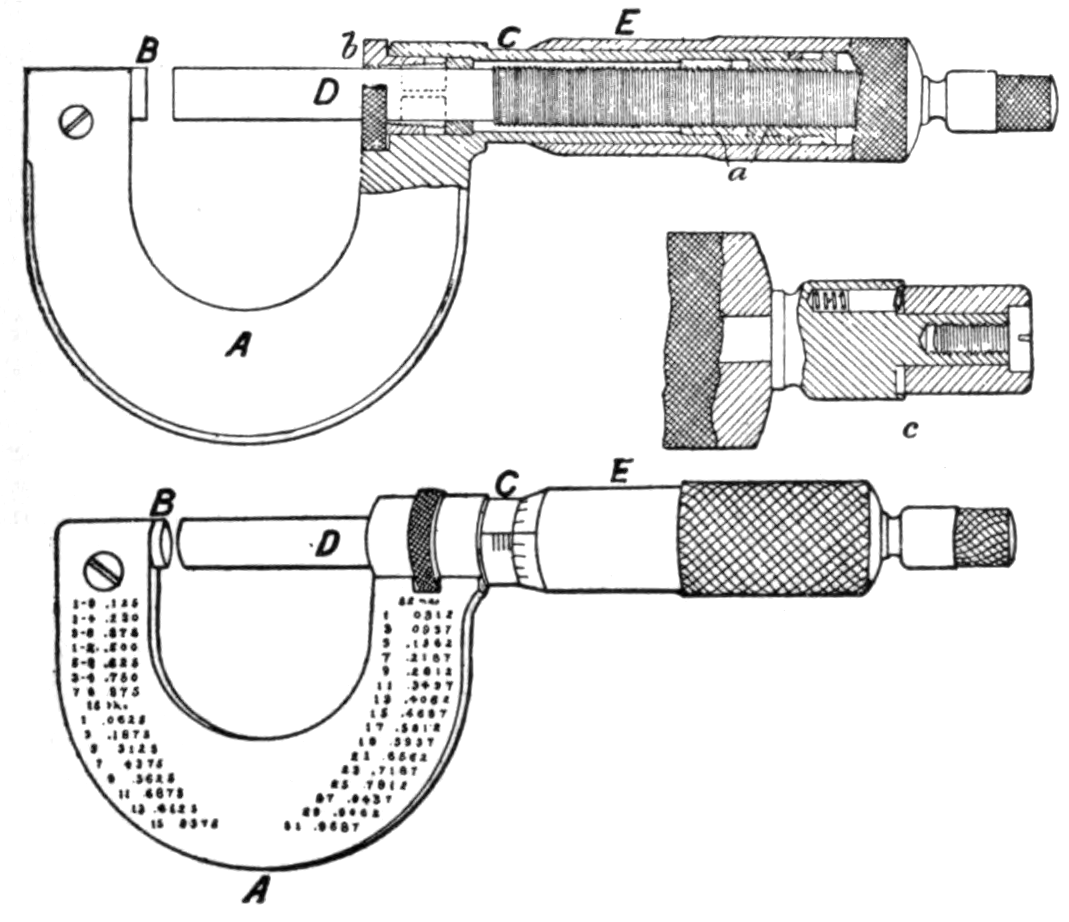
\includegraphics[width=\linewidth, trim={0 16cm 0 0},clip, alt={An technical line drawing from 1911 displaying cross-sectional and exterior views of an outside micrometer caliper with lettered components. The top sectional view reveals the internal threaded spindle mechanism a, locking ring b, main barrel sleeve C, and outer thimble sleeve E attached to frame A between anvil B and spindle D. A detailed cross-section inset labeled c depicts the internal ratchet stop mechanism on the right, while the bottom exterior view shows the assembled micrometer with printed fraction conversion tables along the C-frame face.}]{EB1911_-_Tool_-_Fig_72}

                \vspace{0.5em}
                {\tiny \textbf{Attibution:} Encyclopædia Britannica, Public domain, via \href{https://commons.wikimedia.org/wiki/File:EB1911_-_Tool_-_Fig_72.png}{Wikimedia Commons}, cropped from original\par}
            \end{figure}
        \end{column}
    \end{columns}
\end{frame}

\begin{frame}
	\frametitle{Screw Revolution Reading}

    \begin{columns}
        \begin{column}{0.48\linewidth}
            \begin{itemize}[<+- | alert@+>]
                \item Barrel scale reads full revolutions of the screw
                \item Thimble scale reads partial revolutions of the screw
            \end{itemize}
        \end{column}
        \begin{column}{0.48\linewidth}
            \shadowpic[]{\linewidth}{A extreme close-up view of a micrometer barrel and thimble scale resting on a wooden background. The stationary sleeve features a central datum line with millimeter and half-millimeter graduations numbered 0 through 9, while the rotating thimble on the right displays aligned circumferential scale divisions marked 15 and 20.}{}{BarrelScale}
        \end{column}
    \end{columns}
\end{frame}

\begin{frame}
	\frametitle{Spindle}

    \begin{columns}
        \begin{column}{0.48\linewidth}
            \begin{itemize}[<+- | alert@+>]
                \item Unthreaded part of the screw
                \item Advances/retracts in the frame
                \item Supported by a plain bearing in the barrel
            \end{itemize}
        \end{column}
        \begin{column}{0.48\linewidth}
            \shadowpic[]{\linewidth}{A monochrome labeled diagram of an outside micrometer caliper with black arrows identifying its primary components. Arrows point to the C-shaped frame stamped with decimal equivalents, the fixed anvil, the sliding spindle, the lock nut, the graduated sleeve, and the knurled thimble. Text annotations note alternative names such as barrel or stock for the sleeve, lock-ring or lock lever for the lock nut, and state that the internal screw and optional ratchet stop are not pictured.}{\textbf{Attibution:} Three-quarter-ten, \href{https://creativecommons.org/licenses/by-sa/4.0/}{CC BY-SA 4.0}, via \href{https://commons.wikimedia.org/wiki/File:Micrometer_caliper_parts_0001.png}{Wikimedia Commons}}{Micrometer_caliper_parts_0001}
        \end{column}
    \end{columns}
\end{frame}

\begin{frame}
	\frametitle{Large Micrometer Offset}

    \begin{columns}
        \begin{column}{0.48\linewidth}
            \begin{itemize}[<+- | alert@+>]
                \item \emph{ALL} imperial micrometers are 1" micrometers
                    \begin{itemize}
                        \item A 2" micrometer is still a 1" micrometer
                        \item Spindle only closes to within 1" of anvil
                        \item You need to automatically add 1" to all measurements
                    \end{itemize}
            \end{itemize}
        \end{column}
        \begin{column}{0.48\linewidth}
            \shadowpic[]{0.625\linewidth}{A vintage 1908 illustration showing two machinist operators in bowler hats using an extremely large, heavy-duty outside micrometer to measure a massive circular machine component suspended from a heavy rope hoist. The curved micrometer frame features weight-reducing circular cutouts along its entire length, spanning across the top and bottom outer diameter of the workpiece.}{\textbf{Attibution:} Unknown author, Public domain, via \href{https://commons.wikimedia.org/wiki/File:Micrometer--large--Woodworth_1908_p204.png}{Wikimedia Commons}}{Micrometer--large--Woodworth_1908_p204}
        \end{column}
    \end{columns}
\end{frame}

\begin{frame}
	\frametitle{Barrel Vernier Scale}

    \begin{columns}
        \begin{column}{0.48\linewidth}
            \begin{itemize}[<+- | alert@+>]
                \item Some barrels include a \emph{Vernier} scale for 0.0001" resolution
                \item Top of barrel will be divided into 10 equal spaces
            \end{itemize}
        \end{column}
        \begin{column}{0.48\linewidth}
            \shadowpic[]{\linewidth}{A detailed macro shot showing a vernier scale on the sleeve of a micrometer barrel. Eleven parallel longitudinal lines run horizontally along the sleeve, numbered 0 through 9 on the left end, intersecting perpendicular graduations on the adjacent thimble collar on the right.}{}{VernierScale}
        \end{column}
    \end{columns}
\end{frame}

\begin{frame}
	\frametitle{Ratchet}

    \begin{columns}
        \begin{column}{0.48\linewidth}
            \begin{itemize}[<+- | alert@+>]
                \item Measurement pressure is absolutely critical to precision with micrometers
                \item Many micrometers include a ratchet
            \end{itemize}
        \end{column}
        \begin{column}{0.48\linewidth}
            \shadowpic[]{\linewidth}{A Mitutoyo outside micrometer set against a light background, featuring a green C-shaped frame labeled 0-25 0.01mm, a fixed anvil, a movable spindle, a locking lever, and a sleeve and knurled thimble with graduated measuring scales.}{\textbf{Attibution:} Mauro Cateb, \href{https://creativecommons.org/licenses/by-sa/3.0/}{CC BY-SA 3.0}, via \href{https://commons.wikimedia.org/wiki/File:Micrometer_.jpg}{Wikimedia Commons}}{Micrometer}
        \end{column}
    \end{columns}
\end{frame}

\begin{frame}
	\frametitle{Measuring Pressure}

    \begin{columns}
        \begin{column}{0.48\linewidth}
            \begin{itemize}[<+- | alert@+>]
                \item Thimble used for gross adjustment
                \item Ratchet used for fine adjustment -- slips at correct pressure
            \end{itemize}
        \end{column}
        \begin{column}{0.48\linewidth}
            \shadowpic[]{\linewidth}{A Mitutoyo outside micrometer set against a light background, featuring a green C-shaped frame labeled 0-25 0.01mm, a fixed anvil, a movable spindle, a locking lever, and a sleeve and knurled thimble with graduated measuring scales.}{\textbf{Attibution:} Mauro Cateb, \href{https://creativecommons.org/licenses/by-sa/3.0/}{CC BY-SA 3.0}, via \href{https://commons.wikimedia.org/wiki/File:Micrometer_.jpg}{Wikimedia Commons}}{Micrometer}
        \end{column}
    \end{columns}
\end{frame}

\begin{frame}
	\frametitle{Integrated Ratchet}
    \begin{columns}
        \begin{column}{0.48\linewidth}
            \begin{itemize}[<+- | alert@+>]
                \item May be included as an extension on the back of the thimble
                \item May be integrated into the thimble itself
            \end{itemize}
        \end{column}
        \begin{column}{0.48\linewidth}
            \shadowpic[]{\linewidth}{A Mitutoyo outside micrometer set against a light background, featuring a green C-shaped frame labeled 0-25 0.01mm, a fixed anvil, a movable spindle, a locking lever, and a sleeve and knurled thimble with graduated measuring scales.}{\textbf{Attibution:} Mauro Cateb, \href{https://creativecommons.org/licenses/by-sa/3.0/}{CC BY-SA 3.0}, via \href{https://commons.wikimedia.org/wiki/File:Micrometer_.jpg}{Wikimedia Commons}}{Micrometer}
        \end{column}
    \end{columns}
\end{frame}

\begin{frame}
	\frametitle{Lock Nut Mechanism}

    \begin{columns}
        \begin{column}{0.48\linewidth}
            \shadowpic[]{\linewidth}{A monochrome labeled diagram of an outside micrometer caliper with black arrows identifying its primary components. Arrows point to the C-shaped frame stamped with decimal equivalents, the fixed anvil, the sliding spindle, the lock nut, the graduated sleeve, and the knurled thimble. Text annotations note alternative names such as barrel or stock for the sleeve, lock-ring or lock lever for the lock nut, and state that the internal screw and optional ratchet stop are not pictured.}{\textbf{Attibution:} Three-quarter-ten, \href{https://creativecommons.org/licenses/by-sa/4.0/}{CC BY-SA 4.0}, via \href{https://commons.wikimedia.org/wiki/File:Micrometer_caliper_parts_0001.png}{Wikimedia Commons}}{Micrometer_caliper_parts_0001}
        \end{column}
        \begin{column}{0.48\linewidth}
            \shadowpic[]{\linewidth}{A Mitutoyo outside micrometer set against a light background, featuring a green C-shaped frame labeled 0-25 0.01mm, a fixed anvil, a movable spindle, a locking lever, and a sleeve and knurled thimble with graduated measuring scales.}{\textbf{Attibution:} Mauro Cateb, \href{https://creativecommons.org/licenses/by-sa/3.0/}{CC BY-SA 3.0}, via \href{https://commons.wikimedia.org/wiki/File:Micrometer_.jpg}{Wikimedia Commons}}{Micrometer}
        \end{column}
    \end{columns}
\end{frame}

\subsection{Reading Micrometers}

\begin{frame}
	\frametitle{Barrel Scale Divisions}

    \begin{columns}
        \begin{column}{0.48\linewidth}
            \begin{itemize}[<+- | alert@+>]
                \item The barrel includes a linear scale
                \item Linear scale is divided into 10 major divisions
                \item Major divisions = 0.1"
            \end{itemize}
        \end{column}
        \begin{column}{0.48\linewidth}
            \shadowpic[]{\linewidth}{A extreme close-up view of a micrometer barrel and thimble scale resting on a wooden background. The stationary sleeve features a central datum line with millimeter and half-millimeter graduations numbered 0 through 9, while the rotating thimble on the right displays aligned circumferential scale divisions marked 15 and 20.}{}{BarrelScale}
        \end{column}
    \end{columns}
\end{frame}

\begin{frame}
	\frametitle{Minor Barrel Divisions}
    \begin{columns}
        \begin{column}{0.48\linewidth}
            \begin{itemize}[<+- | alert@+>]
                \item Each major division is divided into 4 equal spaces
                \item 0.1" / 4 = 0.025" per minor division
                    \begin{itemize}
                        \item One full revolution of thimble = one minor division
                    \end{itemize}
            \end{itemize}
        \end{column}
        \begin{column}{0.48\linewidth}
            \shadowpic[]{\linewidth}{A extreme close-up view of a micrometer barrel and thimble scale resting on a wooden background. The stationary sleeve features a central datum line with millimeter and half-millimeter graduations numbered 0 through 9, while the rotating thimble on the right displays aligned circumferential scale divisions marked 15 and 20.}{}{BarrelScale}
        \end{column}
    \end{columns}
\end{frame}

\begin{frame}
	\frametitle{Thimble Divisions}

    \begin{columns}
        \begin{column}{0.48\linewidth}
            \begin{itemize}[<+- | alert@+>]
                \item Split into 25 equal divisions, 0.001" apiece
            \end{itemize}
        \end{column}
        \begin{column}{0.48\linewidth}
            \shadowpic[]{\linewidth}{A close-up view focusing on the thimble collar and vernier lines of a micrometer resting on a wooden surface. The edge of the bevel shows fine graduations aligned with sleeve markings, with numbers 0 and 20 visible on the silver sleeve body.}{}{ThimbleScale}
        \end{column}
    \end{columns}
\end{frame}

\begin{frame}
	\frametitle{Vernier Resolution}
    \begin{columns}
        \begin{column}{0.48\linewidth}
            \begin{itemize}[<+- | alert@+>]
                \item On top of barrel 
                \item 10 equal division = 0.0001" apiece
                \item Read like a vernier scale
            \end{itemize}
        \end{column}
        \begin{column}{0.48\linewidth}
            \shadowpic[]{\linewidth}{A detailed macro shot showing a vernier scale on the sleeve of a micrometer barrel. Eleven parallel longitudinal lines run horizontally along the sleeve, numbered 0 through 9 on the left end, intersecting perpendicular graduations on the adjacent thimble collar on the right.}{}{VernierScale}
        \end{column}
    \end{columns}
\end{frame}

\begin{frame}
	\frametitle{Part Placement}

    \begin{columns}
        \begin{column}{0.48\linewidth}
            \begin{itemize}[<+- | alert@+>]
                \item Close the part to be measured between the spindle and anvil
                    \begin{itemize}
                        \item Remember--pressure matters
                        \item Use the ratchet if available
                    \end{itemize}
            \end{itemize}
        \end{column}
        \begin{column}{0.48\linewidth}
            \shadowpic[]{\linewidth}{A close-up view of a metal micrometer measuring the blade of a small flathead screwdriver held between its anvil and spindle faces. A hand supports the frame while the barrel and thimble scale extend to the right.}{}{MicAndScrewdriver2}
        \end{column}
    \end{columns}
\end{frame}

\begin{frame}
	\frametitle{Reading the Barrel Scale}

    \begin{columns}
        \begin{column}{0.48\linewidth}
            \begin{itemize}[<+- | alert@+>]
                \item The last visible line is the barrel scale measurement
                    \begin{itemize}
                        \item 2 = 0.2"
                        \item One more visible line = 0.025"
                        \item Barrel measurement = 0.225"
                    \end{itemize}
            \end{itemize}
        \end{column}
        \begin{column}{0.48\linewidth}
            \shadowpic[]{\linewidth}{A close-up view of the sleeve and thimble scales on a micrometer taking a measurement. The sleeve displays main graduations exposing up to the 0.200 inch mark along with top vernier lines numbered 1 through 4, while the thimble alignment line points precisely to 10 on the thimble scale.}{}{MicAndScrewdriver3}
        \end{column}
    \end{columns}
\end{frame}

\begin{frame}
	\frametitle{Reading the Thimble Scale}

    \begin{columns}
        \begin{column}{0.48\linewidth}
            \begin{itemize}[<+- | alert@+>]
                \item The Price is Right--the closest without going over is the thimble measurement
                    \begin{itemize}
                        \item 10 is closest to the barrel line
                        \item 10 = 0.010"
                    \end{itemize}
            \end{itemize}
        \end{column}
        \begin{column}{0.48\linewidth}
            \shadowpic[]{\linewidth}{A close-up view of the sleeve and thimble scales on a micrometer taking a measurement. The sleeve displays main graduations exposing up to the 0.200 inch mark along with top vernier lines numbered 1 through 4, while the thimble alignment line points precisely to 10 on the thimble scale.}{}{MicAndScrewdriver3}
        \end{column}
    \end{columns}
\end{frame}

\begin{frame}
	\frametitle{The Total Measurement}
    \begin{columns}
        \begin{column}{0.48\linewidth}
            \begin{itemize}[<+- | alert@+>]
                \item Total measurement = barrel measurement + thimble measurement
                    \begin{itemize}
                        \item 0.225" + 0.010" = 0.235"
                    \end{itemize}
                \item{If the micrometer doesn't include a vernier scale, this is the best that can be measured}
            \end{itemize}
        \end{column}
        \begin{column}{0.48\linewidth}
            \shadowpic[]{\linewidth}{A close-up view of the sleeve and thimble scales on a micrometer taking a measurement. The sleeve displays main graduations exposing up to the 0.200 inch mark along with top vernier lines numbered 1 through 4, while the thimble alignment line points precisely to 10 on the thimble scale.}{}{MicAndScrewdriver3}
        \end{column}
    \end{columns}
\end{frame}

\begin{frame}
	\frametitle{Reading the Vernier Scale (1 of 2)}
    \begin{columns}
        \begin{column}{0.48\linewidth}
            \begin{itemize}[<+- | alert@+>]
                \item Notice the measurement is \emph{almost} to 11 on the thimble
                \item Without a vernier, though, 10 \emph{has} to be the measurement
            \end{itemize}
        \end{column}
        \begin{column}{0.48\linewidth}
            \shadowpic[]{\linewidth}{A close-up view of the sleeve and thimble scales on a micrometer taking a measurement. The sleeve displays main graduations exposing up to the 0.200 inch mark along with top vernier lines numbered 1 through 4, while the thimble alignment line points precisely to 10 on the thimble scale.}{}{MicAndScrewdriver3}
        \end{column}
    \end{columns}
\end{frame}

\begin{frame}
	\frametitle{Reading the Vernier Scale (2 of 2)}

    \begin{columns}
        \begin{column}{0.48\linewidth}
            \begin{itemize}[<+- | alert@+>]
                \item 7 has the best alignment
                    \begin{itemize}
                        \item Which barrel line it matches doesn't matter 
                    \end{itemize}
                \item 7 = 0.0007"
                \item 0.235" + 0.0007" = 0.2357"
            \end{itemize}
        \end{column}
        \begin{column}{0.48\linewidth}
            \shadowpic[]{\linewidth}{A macro close-up view of a micrometer barrel showing vernier lines on the sleeve aligned with circumferential graduations on the thimble. The sleeve displays horizontal vernier markings numbered 0 through 9 on the left, while the thimble bevel on the right shows scale divisions near the 15 and 20 marks.}{}{MicAndScrewdriver5}
        \end{column}
    \end{columns}
\end{frame}

\begin{frame}
	\frametitle{Video: Metric Micrometer}

    \centering
    \href{https://www.youtube.com/watch?v=StBc56ZifMs}{How to Read a Metric Micrometer by WeldNotes.com}

    \vspace{0.5em}
    {\footnotesize \href{https://www.youtube.com/watch?v=StBc56ZifMs}{https://www.youtube.com/watch?v=StBc56ZifMs}\par}

    \vspace{0.5em}
    {\tiny Video \textcopyright WeldNotes via YouTube.com\par}
\end{frame}

\subsection{Types of Micrometers}

\begin{frame}
	\frametitle{Specialized Micrometers}

    \begin{columns}
        \begin{column}{0.48\linewidth}
            \begin{itemize}[<+- | alert@+>]
                \item Many sizes and styles of micrometers
                \item Some specialized for specific measurement tasks
                \item All use the same basic function to perform the measurement
            \end{itemize}
        \end{column}
        \begin{column}{0.48\linewidth}
            \shadowpic[]{0.875\linewidth}{Three metallic micrometer tools shown against a white background, including an outside micrometer at the top with printed decimal equivalent charts on its C-shaped frame, an inside or depth micrometer spindle in the middle, and a depth micrometer with a flat base plate at the bottom.}{\textbf{Attribution:} Splarka at English Wikipedia, Public domain, via \href{https://commons.wikimedia.org/wiki/File:Micrometers.jpg}{Wikimedia Commons}}{Micrometers}
        \end{column}
    \end{columns}
\end{frame}

\begin{frame}
	\frametitle{Outside Micrometers}

    \begin{columns}
        \begin{column}{0.48\linewidth}
            \begin{itemize}[<+- | alert@+>]
                \item The micrometers we've been looking at
                \item Used to measure outside dimensions of parts
                \item Available in different sizes
                    \begin{itemize}
                        \item Remember: bigger micrometers still only have 1" of stroke
                    \end{itemize}
            \end{itemize}
        \end{column}
        \begin{column}{0.48\linewidth}
            \shadowpic[]{\linewidth}{A Mitutoyo outside micrometer set against a light background, featuring a green C-shaped frame labeled 0-25 0.01mm, a fixed anvil, a movable spindle, a locking lever, and a sleeve and knurled thimble with graduated measuring scales.}{\textbf{Attibution:} Mauro Cateb, \href{https://creativecommons.org/licenses/by-sa/3.0/}{CC BY-SA 3.0}, via \href{https://commons.wikimedia.org/wiki/File:Micrometer_.jpg}{Wikimedia Commons}}{Micrometer}
        \end{column}
    \end{columns}
\end{frame}

\begin{frame}
	\frametitle{Telescoping Gauges}

    \begin{columns}
        \begin{column}{0.48\linewidth}
            \begin{itemize}[<+- | alert@+>]
                \item{Not a mircometer -- commonly used with outside micrometers}
                \item{Two expanding rods}
                \item{Screw in handle extends/retracts rods}
                \item{Gauge expanded to walls of part -- transferred to outside micrometer for measurement}
            \end{itemize}
        \end{column}
        \begin{column}{0.48\linewidth}
            \shadowpic[]{\linewidth}{A set of six metallic Starrett telescoping gauges arranged in individual pockets inside a bright red protective vinyl case. Each T-shaped gauge consists of a knurled handle with a knurled locking screw and spring-loaded telescoping plungers of varying widths, with labeled size ranges printed on the pockets below ranging from 5/16 inch to 6 inches, or 8 mm to 152 mm.}{\textbf{Attibution:} Nathanael Burton, \href{https://creativecommons.org/licenses/by-sa/2.0/}{CC BY-SA 2.0}, via \href{https://commons.wikimedia.org/wiki/File:Set_of_Six_Starrett_Telescoping_Gages_No.S579H.jpg}{Wikimedia Commons}}{Set_of_Six_Starrett_Telescoping_Gages_No.S579H}
        \end{column}
    \end{columns}
\end{frame}

\begin{frame}
	\frametitle{Thread Micrometer}
    \begin{columns}
        \begin{column}{0.48\linewidth}
            \begin{itemize}[<+- | alert@+>]
                \item Special outside micrometer
                \item Measures screw minor diameter
                \item Anvil and spindle are pointed to get between screw threads
            \end{itemize}
        \end{column}
        \begin{column}{0.48\linewidth}
            \shadowpic[]{\linewidth}{A close-up view of a specialized screw thread micrometer with a blue speckled frame measuring the pitch diameter of a threaded steel shaft. The v-shaped anvil on the left cradles a single thread crest while the pointed cone spindle tip on the right seats directly into an opposing thread groove. The black frame plate indicates a range of 25 to 50 mm with 0.01 mm graduations rated at 20 degrees Celsius.}{\textbf{Attibution:} Christoph Baumgartinger, \href{https://creativecommons.org/licenses/by-sa/2.5/}{CC BY-SA 2.5}, via \href{https://commons.wikimedia.org/wiki/File:Thread_Micrometer_Detail.jpg}{Wikimedia Commons}}{Thread_Micrometer_Detail}
        \end{column}
    \end{columns}
\end{frame}

\begin{frame}
	\frametitle{Inside Micrometers}

    \begin{columns}
        \begin{column}{0.48\linewidth}
            \begin{itemize}[<+- | alert@+>]
                \item Used to measure inside dimensions of parts
            \end{itemize}
        \end{column}
        \begin{column}{0.48\linewidth}
            \shadowpic[]{\linewidth}{Two Mitutoyo caliper-type inside micrometers displayed horizontally against a plain gray background. The top unit features outward-facing measuring nibs with a labeled range of 5 to 30 mm, while the bottom unit features offset hooked jaws with a range of 25 to 50 mm, both equipped with graduated thimbles and knurled adjustment ratchets.}{\textbf{Attibution:} Glenn McKechnie, \href{https://creativecommons.org/licenses/by-sa/2.0/}{CC BY-SA 2.0}, via \href{https://commons.wikimedia.org/wiki/File:MicrometerInside5-30_25-50.jpg}{Wikimedia Commons}}{MicrometerInside5-30_25-50}
        \end{column}
    \end{columns}
\end{frame}

\begin{frame}
	\frametitle{Depth Micrometer}
    \begin{columns}
        \begin{column}{0.48\linewidth}
            \begin{itemize}[<+- | alert@+>]
                \item Used to measure the depth of holes/pockets
                \item Frame is a single, flat surface to rest on part
                \item No fixed anvil
                \item Spindle is usually interchangeable for different starting depths
            \end{itemize}
        \end{column}
        \begin{column}{0.48\linewidth}
            \shadowpic[]{0.75\linewidth}{A Mitutoyo depth micrometer with a flat ground base resting vertically alongside an interchangeable measuring rod on a gray surface. The main body features a wide base plate labeled Mitutoyo 0.01mm, model number 916947, Made in Japan, surmounted by a graduated vertical sleeve and knurled thimble. The separate measuring rod on the left has a capped end collar designed for insertion through the central spindle sleeve.}{\textbf{Attibution:} Glenn McKechnie, \href{https://creativecommons.org/licenses/by-sa/2.0/}{CC BY-SA 2.0}, via \href{https://commons.wikimedia.org/wiki/File:MicrometerDepth916947.jpg}{Wikimedia Commons}}{MicrometerDepth916947}
        \end{column}
    \end{columns}
\end{frame}

\begin{frame}
    \centering
    {\Huge \textbf{\textcolor{BakerADARed}{Questions?}}}
\end{frame}

\begin{frame}
    \frametitle{Copyright Notice}

    % \begin{figure}
    %     \centering
    %     
\includegraphics[width=0.25\linewidth, alt={Creative Commons Attribution NonCommercial ShareAlike logo displaying four circular icons arranged horizontally over a black banner. From left to right, the icons feature the CC logo, a person pictogram for Attribution labeled BY below, a slashed dollar sign for NonCommercial labeled NC below, and a counterclockwise circular arrow for ShareAlike labeled SA below.}]{by-nc-sa.png}
    % \end{figure}
    
    {\footnotesize
    \PresTitle \textcopyright 2026 by Brad Peirson is licensed under Creative Commons Attribution-NonCommercial-ShareAlike 4.0 International (CC BY-NC-SA 4.0). To view a copy of the official license, visit \href{https://creativecommons.org/licenses/by-nc-sa/4.0/}{https://creativecommons.org/licenses/by-nc-sa/4.0/}.

    \vspace{0.5em}

    \textbf{Exceptions and Exclusions}

    \begin{itemize}
        \item[Baker College Branding \& Trademarks:]All Baker College logos, trademarks, wordmarks, seals, slide design templates, and proprietary branding elements contained in these materials are \textbf{EXCLUDED} from the CC BY-NC-SA 4.0 license. All rights are reserved by Baker College. Express written permission from Baker College is required for any use, copying, or redistribution of these elements.
        \item[Third-Party Media \& Content:] Any third-party images, graphics, diagrams, or external media incorporated in these materials are included under their respective original licenses or permissions and are individually attributed at their point of use. 
        \item[Original Author Content:] All unattributed figures, diagrams, text, code snippets, and media are original works created by the author and are licensed under the CC BY-NC-SA 4.0 license.
    \end{itemize}
    \par}
\end{frame}

\end{document}

% \begin{frame}
%     \frametitle{Test Todo}

%     % Usage: \tikztodo[width]{height}{description/notes}
%     \tikztodo[0.7\textwidth]{4cm}{Convert block diagram of feedback loop}
% \end{frame}